% Options for packages loaded elsewhere
\PassOptionsToPackage{unicode}{hyperref}
\PassOptionsToPackage{hyphens}{url}
\PassOptionsToPackage{dvipsnames,svgnames,x11names}{xcolor}
%
\documentclass[
]{jds}

\usepackage{amsmath,amssymb}
\usepackage{lmodern}
\usepackage{iftex}
\ifPDFTeX
  \usepackage[T1]{fontenc}
  \usepackage[utf8]{inputenc}
  \usepackage{textcomp} % provide euro and other symbols
\else % if luatex or xetex
  \usepackage{unicode-math}
  \defaultfontfeatures{Scale=MatchLowercase}
  \defaultfontfeatures[\rmfamily]{Ligatures=TeX,Scale=1}
\fi
% Use upquote if available, for straight quotes in verbatim environments
\IfFileExists{upquote.sty}{\usepackage{upquote}}{}
\IfFileExists{microtype.sty}{% use microtype if available
  \usepackage[]{microtype}
  \UseMicrotypeSet[protrusion]{basicmath} % disable protrusion for tt fonts
}{}
\makeatletter
\@ifundefined{KOMAClassName}{% if non-KOMA class
  \IfFileExists{parskip.sty}{%
    \usepackage{parskip}
  }{% else
    \setlength{\parindent}{0pt}
    \setlength{\parskip}{6pt plus 2pt minus 1pt}}
}{% if KOMA class
  \KOMAoptions{parskip=half}}
\makeatother
\usepackage{xcolor}
\setlength{\emergencystretch}{3em} % prevent overfull lines
\setcounter{secnumdepth}{-\maxdimen} % remove section numbering
% Make \paragraph and \subparagraph free-standing
\ifx\paragraph\undefined\else
  \let\oldparagraph\paragraph
  \renewcommand{\paragraph}[1]{\oldparagraph{#1}\mbox{}}
\fi
\ifx\subparagraph\undefined\else
  \let\oldsubparagraph\subparagraph
  \renewcommand{\subparagraph}[1]{\oldsubparagraph{#1}\mbox{}}
\fi


\providecommand{\tightlist}{%
  \setlength{\itemsep}{0pt}\setlength{\parskip}{0pt}}\usepackage{longtable,booktabs,array}
\usepackage{calc} % for calculating minipage widths
% Correct order of tables after \paragraph or \subparagraph
\usepackage{etoolbox}
\makeatletter
\patchcmd\longtable{\par}{\if@noskipsec\mbox{}\fi\par}{}{}
\makeatother
% Allow footnotes in longtable head/foot
\IfFileExists{footnotehyper.sty}{\usepackage{footnotehyper}}{\usepackage{footnote}}
\makesavenoteenv{longtable}
\usepackage{graphicx}
\makeatletter
\def\maxwidth{\ifdim\Gin@nat@width>\linewidth\linewidth\else\Gin@nat@width\fi}
\def\maxheight{\ifdim\Gin@nat@height>\textheight\textheight\else\Gin@nat@height\fi}
\makeatother
% Scale images if necessary, so that they will not overflow the page
% margins by default, and it is still possible to overwrite the defaults
% using explicit options in \includegraphics[width, height, ...]{}
\setkeys{Gin}{width=\maxwidth,height=\maxheight,keepaspectratio}
% Set default figure placement to htbp
\makeatletter
\def\fps@figure{htbp}
\makeatother
\newlength{\cslhangindent}
\setlength{\cslhangindent}{1.5em}
\newlength{\csllabelwidth}
\setlength{\csllabelwidth}{3em}
\newlength{\cslentryspacingunit} % times entry-spacing
\setlength{\cslentryspacingunit}{\parskip}
\newenvironment{CSLReferences}[2] % #1 hanging-ident, #2 entry spacing
 {% don't indent paragraphs
  \setlength{\parindent}{0pt}
  % turn on hanging indent if param 1 is 1
  \ifodd #1
  \let\oldpar\par
  \def\par{\hangindent=\cslhangindent\oldpar}
  \fi
  % set entry spacing
  \setlength{\parskip}{#2\cslentryspacingunit}
 }%
 {}
\usepackage{calc}
\newcommand{\CSLBlock}[1]{#1\hfill\break}
\newcommand{\CSLLeftMargin}[1]{\parbox[t]{\csllabelwidth}{#1}}
\newcommand{\CSLRightInline}[1]{\parbox[t]{\linewidth - \csllabelwidth}{#1}\break}
\newcommand{\CSLIndent}[1]{\hspace{\cslhangindent}#1}

\usepackage{booktabs}
\usepackage{caption}
\usepackage{longtable}
\usepackage{lscape}
\author[1]{Kiegan Rice\thanks{Corresponding author. Email: rice-kiegan@norc.org}}
\author[2]{Heike Hofmann\footnote{Email: hofmann@iastate.edu}}
\author[1]{Nola du Toit\footnote{Email: dutoit-nola@norc.org}}
\author[1]{Edward Mulrow\footnote{Email: mulrow-edward@norc.org}}
\affil[1]{NORC at the University of Chicago}
\affil[2]{Department of Statistics, Iowa State University}
\makeatletter
\makeatother
\makeatletter
\makeatother
\makeatletter
\@ifpackageloaded{caption}{}{\usepackage{caption}}
\AtBeginDocument{%
\ifdefined\contentsname
  \renewcommand*\contentsname{Table of contents}
\else
  \newcommand\contentsname{Table of contents}
\fi
\ifdefined\listfigurename
  \renewcommand*\listfigurename{List of Figures}
\else
  \newcommand\listfigurename{List of Figures}
\fi
\ifdefined\listtablename
  \renewcommand*\listtablename{List of Tables}
\else
  \newcommand\listtablename{List of Tables}
\fi
\ifdefined\figurename
  \renewcommand*\figurename{Figure}
\else
  \newcommand\figurename{Figure}
\fi
\ifdefined\tablename
  \renewcommand*\tablename{Table}
\else
  \newcommand\tablename{Table}
\fi
}
\@ifpackageloaded{float}{}{\usepackage{float}}
\floatstyle{ruled}
\@ifundefined{c@chapter}{\newfloat{codelisting}{h}{lop}}{\newfloat{codelisting}{h}{lop}[chapter]}
\floatname{codelisting}{Listing}
\newcommand*\listoflistings{\listof{codelisting}{List of Listings}}
\makeatother
\makeatletter
\@ifpackageloaded{caption}{}{\usepackage{caption}}
\@ifpackageloaded{subcaption}{}{\usepackage{subcaption}}
\makeatother
\makeatletter
\@ifpackageloaded{tcolorbox}{}{\usepackage[many]{tcolorbox}}
\makeatother
\makeatletter
\@ifundefined{shadecolor}{\definecolor{shadecolor}{rgb}{.97, .97, .97}}
\makeatother
\makeatletter
\makeatother
\ifLuaTeX
  \usepackage{selnolig}  % disable illegal ligatures
\fi
\IfFileExists{bookmark.sty}{\usepackage{bookmark}}{\usepackage{hyperref}}
\IfFileExists{xurl.sty}{\usepackage{xurl}}{} % add URL line breaks if available
\urlstyle{same} % disable monospaced font for URLs
\hypersetup{
  pdftitle={Testing Charts: viewers' perceptual accuracy in surveys},
  pdfkeywords={graphical perception, data visualization, survey data},
  colorlinks=true,
  linkcolor={blue},
  filecolor={Maroon},
  citecolor={Blue},
  urlcolor={Blue},
  pdfcreator={LaTeX via pandoc}}

\title{Testing Charts: viewers' perceptual accuracy in surveys}
\author{}
\date{}

\begin{document}
\maketitle
\begin{abstract}
The use of visuals is a key component in scientific communication.
Decisions about the design of a data visualization should be informed by
what design elements best support the audience's ability to perceive and
understand the components of the data visualization. We build on the
foundations of Cleveland and McGill's work in graphical perception,
employing a large, nationally-representative, probability-based panel of
survey respondents to test perception in statistical charts. Our
findings provide actionable guidance for data visualization
practitioners to employ in their work.
\end{abstract}
\ifdefined\Shaded\renewenvironment{Shaded}{\begin{tcolorbox}[interior hidden, borderline west={3pt}{0pt}{shadecolor}, boxrule=0pt, enhanced, breakable, sharp corners, frame hidden]}{\end{tcolorbox}}\fi

  \newcommand{\hh}[1]{{\textcolor{orange}{#1}}} 
  \newcommand{\kr}[1]{{\textcolor{teal}{#1}}}.  
  \newcommand{\ejm}[1]{{\textcolor{ForestGreen}{#1}}}.  
  \newcommand{\ndt}[1]{{\textcolor{purple}{#1}}}.  

% take out everything above later
% keep everything below

  \newcommand{\blandscape}{\begin{landscape}} 
  \newcommand{\elandscape}{\end{landscape}}

  \setlength{\parindent}{0pt}
  \singlespacing

\hypertarget{introduction}{%
\subsection{Introduction}\label{introduction}}

What do viewers see when we show them a data chart? A data chart -- at
its core -- maps values to graphical elements: quantitative elements are
represented as measurable features, such as position, size, or shade.
Modern data visualizations are much more than a simple, objective
mapping of values to a plane; they contain contextual and design
elements, and are often structured to support the viewer in
understanding a particular view of a set of data or specific pattern
underlying the values. Structural choices, such as the choice of a
graphical element (e.g., bar or pie), orientation of the chart, and
sizing and relative positioning of elements within the chart, are
determined by the data visualization practitioner. The design of a data
visualization impacts a viewer's ability to achieve the intended
understanding; a poorly designed data visualization may leave viewers
struggling to understand the content or context, or make it difficult to
complete accurate and useful comparisons of values across groups or time
points. More broadly, the design of a data visualization can change how
viewers interact with the chart.

The viewer's employment of comparisons of the components is a crucial
step in the process of interacting with and understanding the chart.
Cleveland and McGill (1984) observed as such, and in their seminal study
defined the better visual among a pair as the one that allows viewers to
make more accurate comparisons. Based on mappings of quantitative
variables to different graphical elements, Cleveland and McGill's study
resulted in a ranking of perceptual tasks (such as identifying the
larger of two lengths or areas) from most accurate to least accurate,
which was then extended by Mackinlay (1986) to a theoretical framework
ranking tasks' order along their ordinal and nominal scales.

Cleveland and McGill's work -- while a foundational user study in
graphical perception -- utilized a small convenience sample, consisting
of only a few individuals recruited from among the authors' coworkers
and their spouses. Heer and Bostock (2010) reproduced Cleveland and
McGill's rankings using a larger sample from a crowd sourcing platform,
employing a total of 82 Amazon Mechanical Turk (mTurk) workers for the
study. Crowd sourced samples were shown by Borgo et al. (2017) to be
biased towards more male, younger, and relatively higher education
relative to the adult U.S. population as a whole; generally, convenience
and opt-in samples are not representative of the general population, a
common target audience for data visualization and scientific
communication work. Further, the populations' emphasis on higher
education individuals also leads to results which hold for groups of
individuals who may be more likely to have prior exposure to data
visualization in the context of scientific communication, or more
exposure to data topics in higher education, but may not hold across
other groups within the population.

Here, we seek to answer whether it is possible to reproduce some of the
previous findings in the context of a survey with a large,
nationally-representative set of respondents. Specifically, we present
viewers with structural variations of bar charts and ask them to answer
questions comparing the size of elements within those charts. We employ
a probability-based survey panel and run a series of perception tests
with nationally-representative samples of respondents from that panel.
The advantage of using a probability-based approach is two-fold. First,
we have access to a large sample of survey participants and thus have
greater power in making inference about graphical perceptional
abilities. Second, the sample is representative of the general adult
public in the U.S., and this allows us to test whether prior results
from convenience samples hold with a nationally representative sample
and whether there are differences in those results across demographic
subgroups. Within that context we focus on the following research
questions:

\begin{enumerate}
\def\labelenumi{\arabic{enumi}.}
\item
  How do structural design choices in a data visualization impact
  viewers' ability to identify the larger of two elements?
\item
  How is viewer interaction with the task impacted by structural design
  choices in a data visualization?
\item
  Are there differences in perception and interaction with the tasks
  across demographic groups?
\end{enumerate}

In this work, we present a series of completed tests and the resulting
findings. The remainder of the paper is organized as follows: first, we
describe the design of the visual stimuli used in the perception tests.
We then describe the population of study respondents and obtained survey
sample. Subsequently, we share a summary of the resulting survey
responses across each of the tests, including analyses on accuracy of
responses and response behavior. Finally, we discuss implications of
this work and next steps.

\hypertarget{study-design-stimulus}{%
\subsection{Study design -- stimulus}\label{study-design-stimulus}}

Our use of a survey format guides the format and design of the questions
asked and how they are presented to respondents. First, participant
instructions must be delivered in a very short and easily understandable
format, because participants cannot ask clarifying questions about the
task as they might be able to in a cognitive lab setting. Our tasks are
presented as a short series of questions within a larger survey on a
variety of topics. Second, we want to utilize content within the
stimulus which is not socially or politically charged for the average
U.S. adult; this risks participants reacting to the subject matter
within the chart rather than focusing on the task. For this reason, we
utilize data on living arrangements of older U.S. adults -- a topic
which most U.S. adults will have some familiarity with, but is not
inherently polarizing. Finally, to prevent viewers from being exposed to
slight variations of the same stimulus in a row (and risk unforeseen
order effects or respondents using prior questions to inform their
responses), we either split a survey sample in two and show each
subsample a distinct structural version of the chart or test variations
of a chart across distinct rounds of the survey.

Each task is made up of two elements: a visual stimulus and a question
about the stimulus. In our study, each visual stimulus is an image of a
data visualization, while each question prompts viewers to identify
which of two marked pieces in the data visualization is larger.

The comparison between sets of marked pairs is intentionally designed to
be a difficult task, with the difference between the values represented
in the two marked pieces being chosen close to their just-noticeable
difference. The \textbf{Just-Noticeable Difference} (JND) is defined as
the smallest difference that will be detected 50\% of the time. Prior
results from studies on bar charts and pie charts (Lu et al. 2022)
inform the differences in charts shown to survey panelists.

We employ comparisons at the JND in our tasks in order to maximize our
ability to identify the impact of design changes on viewer accuracy and
behavior. Asking perception tasks in a survey differs from the
controlled environment of a cognitive lab, where these kind of questions
may usually be assessed. Rather than asking the same (or similar) type
of question with varied signal strength dozens or hundreds of times, we
are limited to only a few questions at a time. With a small set of
tasks, we need to present tasks that are perceptually hard, and thus ask
questions about stimuli that are close to our perceptual threshold.
Therefore, we focus on questions which vary the structure of the
presented image, but ask viewers to compare the same underlying data
values across those varied images.

We ask participants to determine which of two just-noticeably different
marked pieces (tiles) is larger within each chart, and focus on three
main sets of structural variation in the design of that chart:

\begin{itemize}
\item
  First, we vary the alignment of the pieces in question. Viewers are
  presented with two marked pieces in a chart that do not share a common
  baseline (aligned pieces), then two pieces that do share a common
  baseline (unaligned pieces).
\item
  Second, we vary the orientation of the chart -- we rotate the vertical
  stacked bar chart, and present a horizontally oriented version of the
  same chart, with identically sized marked pieces.
\item
  Finally, we change the aspect ratio of the chart and present a wider
  version of the horizontally oriented chart which has longer, but
  thinner, marked pieces.
\end{itemize}

\begin{figure*}[hbt]

{\centering 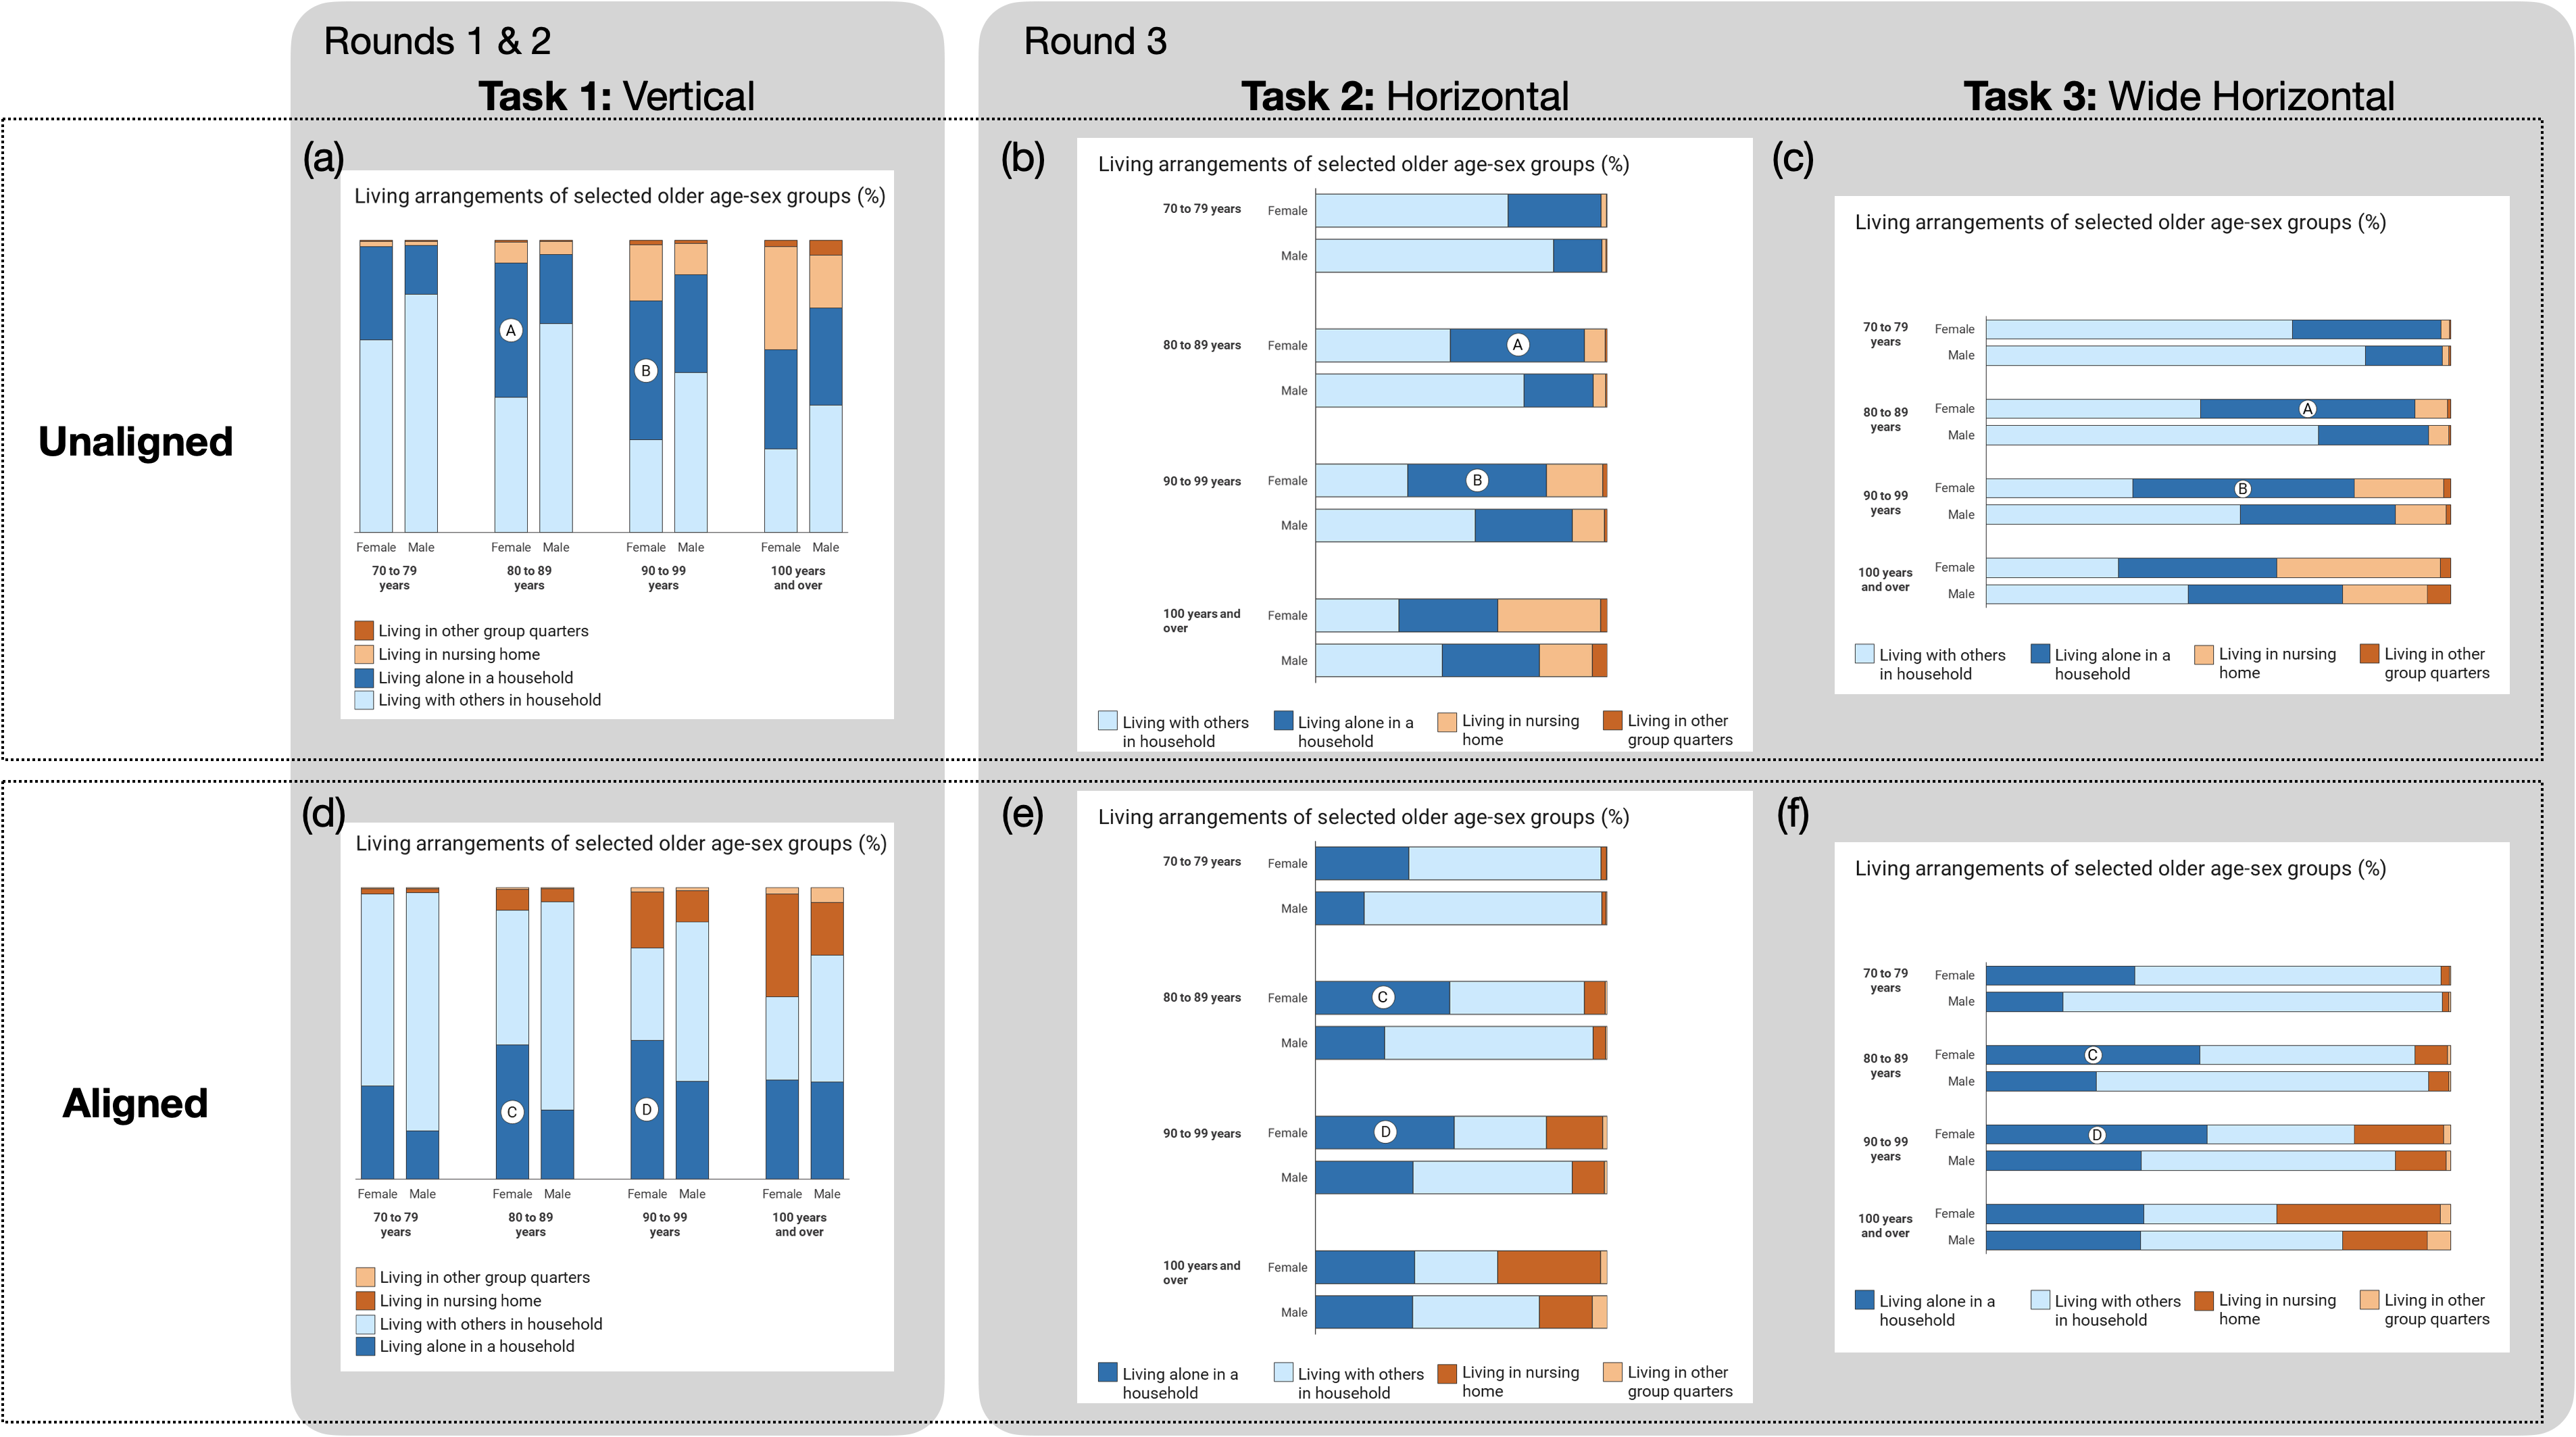
\includegraphics[width=0.9\textwidth,height=\textheight]{images/stimuli-overview.png}

}

\caption{\label{fig-tasks}Each of the visual stimuli presented to
viewers. In each bar chart, two pieces are marked. The larger piece in
each chart are pieces B and D.}

\end{figure*}

\hypertarget{task-1-vertical-stacked-bar}{%
\subsubsection{Task 1: Vertical stacked
bar}\label{task-1-vertical-stacked-bar}}

\autoref{fig-tasks}(a,d) shows the two stacked bar charts shown to
participants in the first task. The marked tiles in each plot are 155
pixels apart, which leads to a JND of 3.5 pixels based on Lu et al.
(2022)`s model. The heights of the bars are 205 (left) and 213 pixels
(right), corresponding to about twice the JND. This difference should
lead to a relatively high accuracy rate for participants and
simultaneously limit the amount of frustration resulting from a task
that is perceived as `too hard'.

Both charts show the same data with slight modifications to the order of
the levels -- the first and second level in each of the bars are
reversed between the chart in (a) and the chart in (d). Both charts are
displayed at the same size, i.e.~in both cases both the difference in
size between the bars and the horizontal distance between the bars is
the exact same amount. This leaves the vertical positioning of the bars
as the only difference between the charts. Any differences in observed
responses can therefore be attributed to this difference in
presentation.

\hypertarget{task-2-horizontal-stacked-bar}{%
\subsubsection{Task 2: Horizontal stacked
bar}\label{task-2-horizontal-stacked-bar}}

The visual mappings in the second task, shown in
\autoref{fig-tasks}(b,e), are identical to the first task, but the axes
of the chart are rotated so that the stacked bars are represented in a
horizontal format. This represents a structural change in how the data
are presented to the viewer while preserving the pixel size of the
elements viewers must compare. Tasks 2 and 3 were asked within the same
survey round (Round 3) and the full sample was randomly split among
respondents, with 50\% of participants seeing the Task 2 stimuli and
50\% of participants seeing the Task 3 stimuli.

\hypertarget{task-3-horizontal-wide-stacked-bar}{%
\subsubsection{Task 3: Horizontal wide stacked
bar}\label{task-3-horizontal-wide-stacked-bar}}

The images utilized in the third task, \autoref{fig-tasks}(c,f), again
represent the same data as in the first two tasks, and the overall image
has dimensions which are identical to the images in the first two tasks,
displaying at the same size during the survey. However, the aspect ratio
is adjusted to make the plotting area match that of Task 1, with the
mapping area being wider rather than taller. The length of bars is
increased to fit the new dimensions. This increases the difference in
the length of bars to 13 pixels (previously 8 pixels). The widths of the
tiles are adjusted accordingly (from 50 to 30 pixels) to keep the
overall area of the tiles approximately constant.

\hypertarget{question-text}{%
\paragraph{Question text}\label{question-text}}

When viewing each chart, participants were asked to compare the relative
sizes of marked elements within the chart:

``There are many charts used in the news media to portray data visually.
Looking at the chart below, which of the marked dark blue pieces is
bigger, A or B? Just your best guess is fine.

\begin{itemize}
\item
  A is bigger
\item
  B is bigger
\item
  They are the same''
\end{itemize}

When presented with the aligned version of each chart, pieces were
marked with a C and D and the question text is updated accordingly. In
all scenarios, the second option (B {[}D{]} is bigger) is the correct
response.

For a given task, viewers are first presented with the unaligned version
of the task, followed by the aligned version of the task. The time in
seconds that each respondent spent on each task was recorded, as well as
whether the participant zoomed in on each chart while answering the
question. Respondents were also asked to rate their certainty in their
response to each question on a five-point scale.

\begin{figure*}[hbt]

{\centering 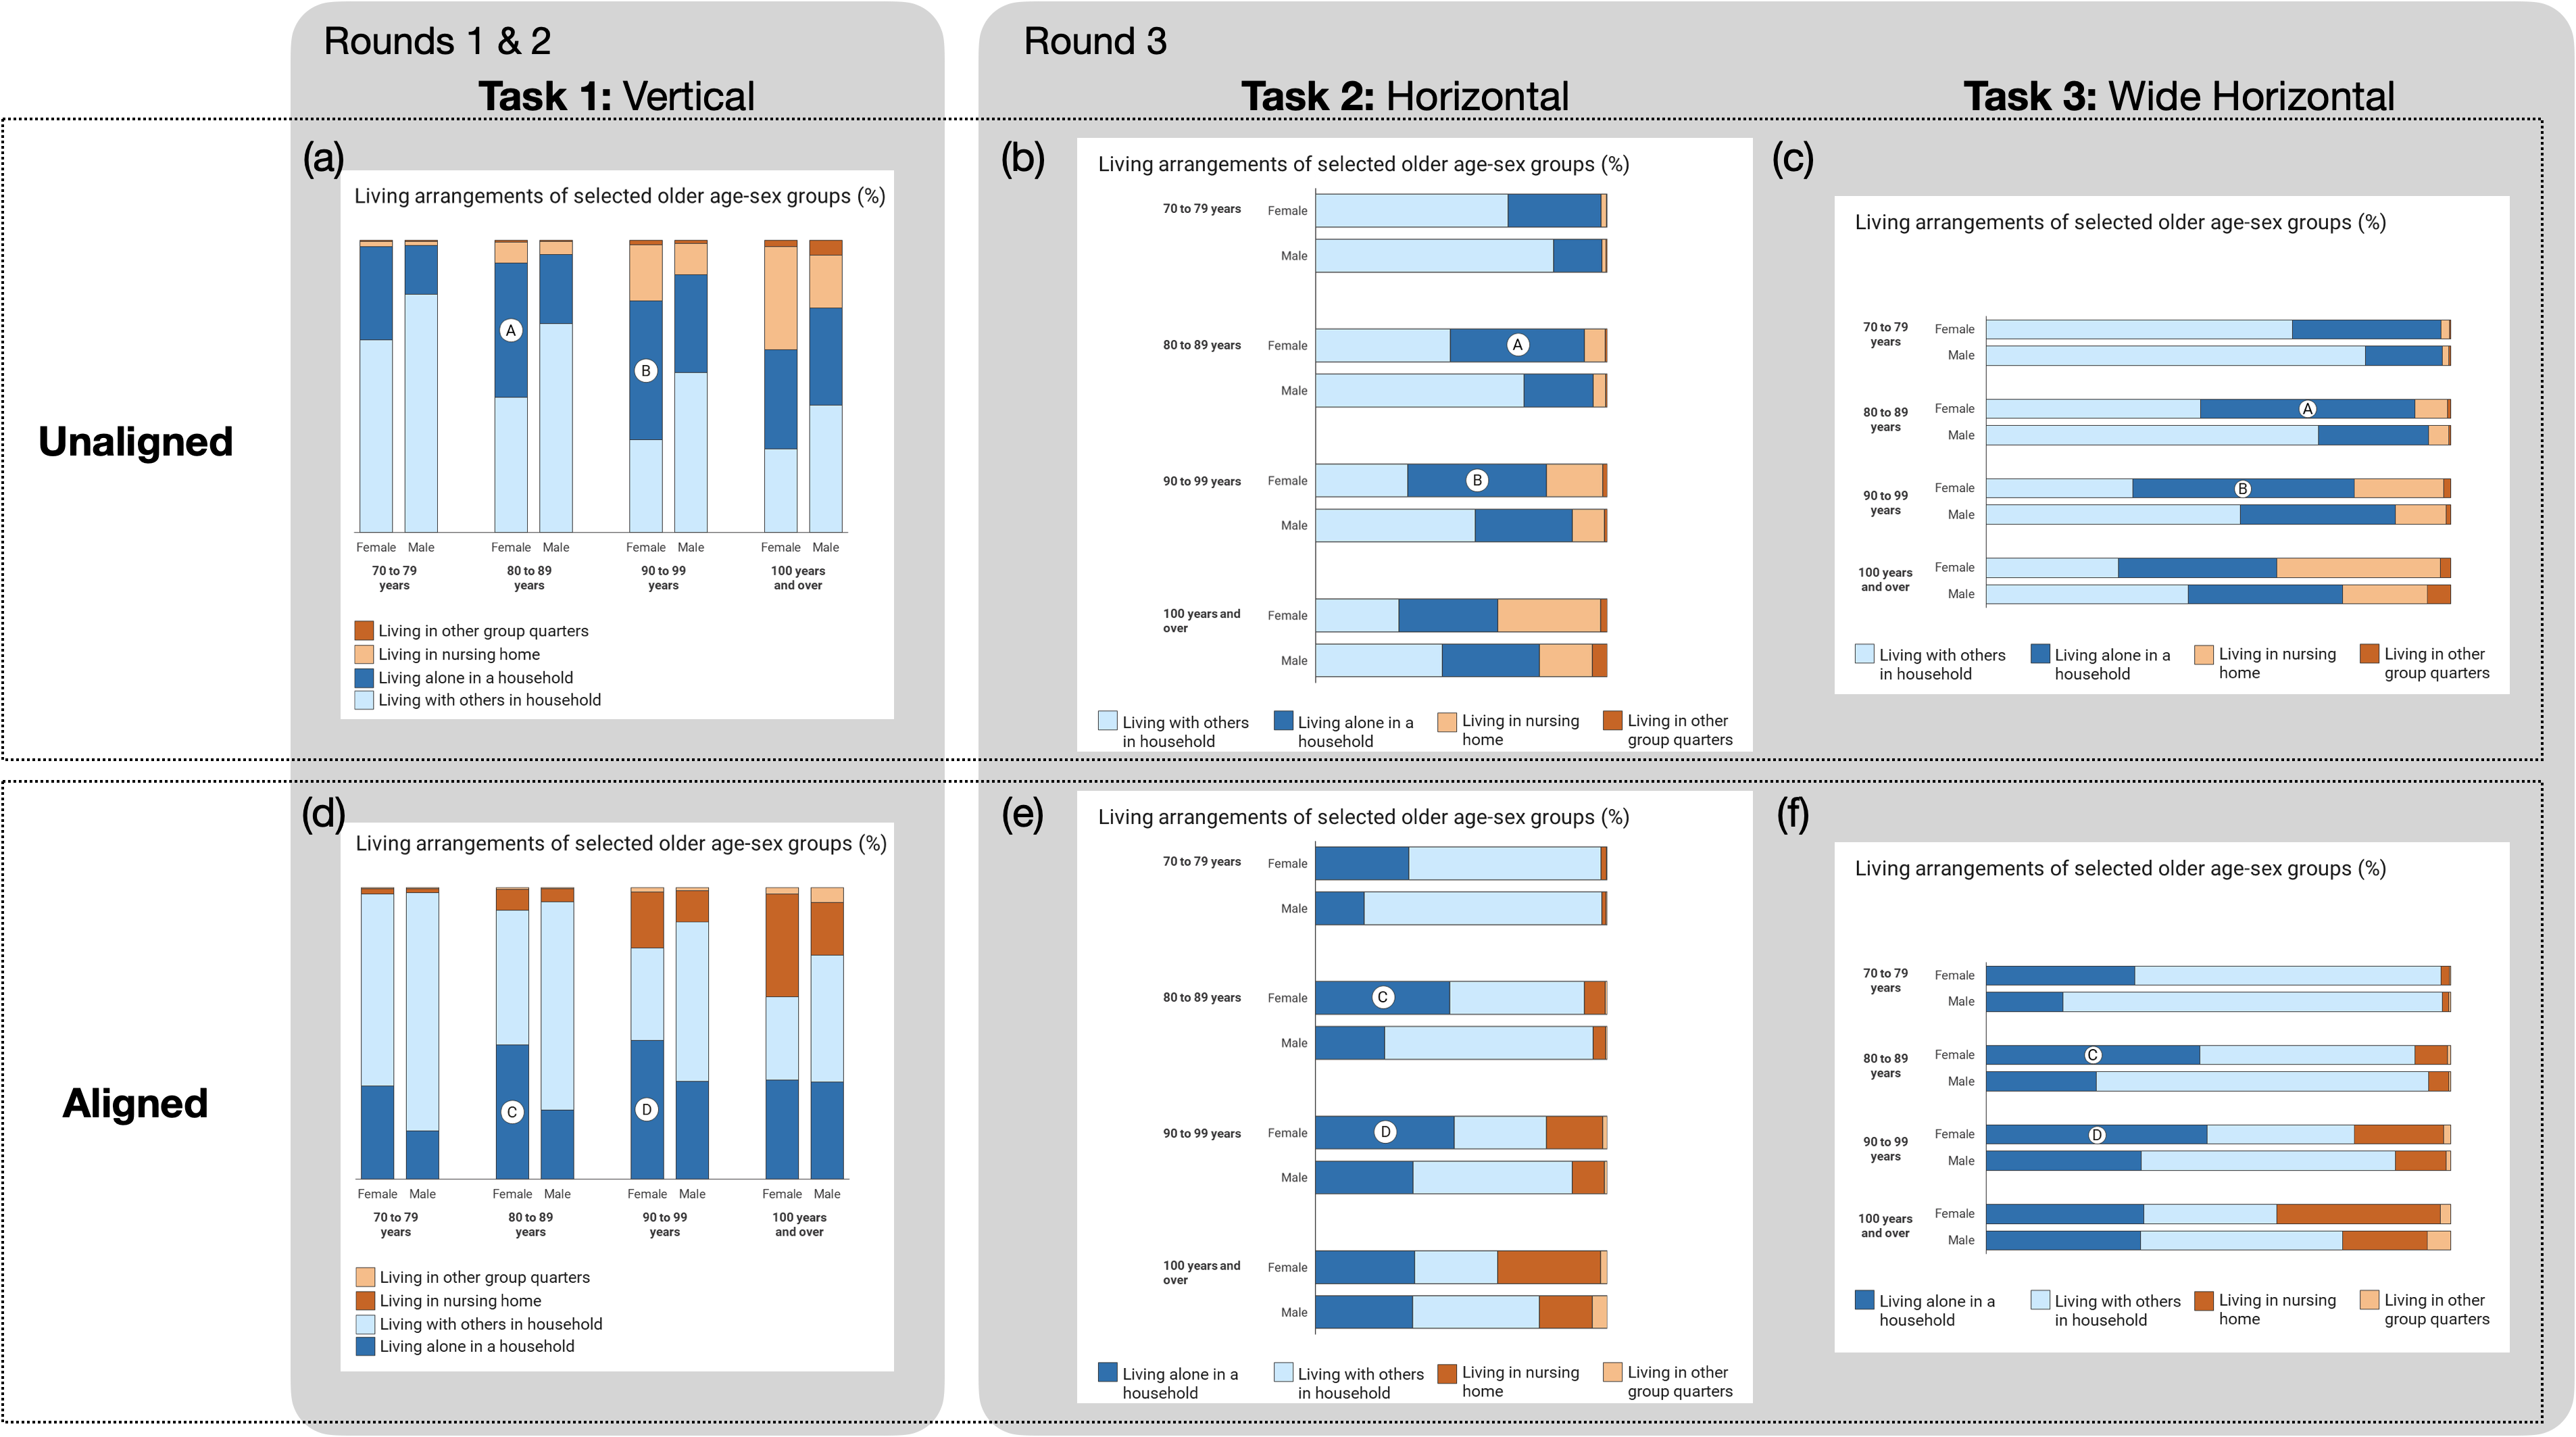
\includegraphics[width=0.6\textwidth,height=\textheight]{images/sketch-tasks.png}

}

\caption{\label{fig-tasks-explain}Comparisons made in charts within the
Cleveland and McGill ranking (left) and their corresponding
representations in our study tasks (right).}

\end{figure*}

\hypertarget{alignment}{%
\paragraph{Alignment}\label{alignment}}

What we call `aligned' and `unaligned', here, is similar to Cleveland
and McGill's positions along aligned and unaligned scales, but with some
modifications. Figure~\ref{fig-tasks-explain} gives an overview of the
comparisons of tasks 1 through 3 and the closest corresponding tasks in
Cleveland and McGill. In this paper, both `aligned' and `unaligned' bars
share the same axis.

Aligned tiles are additionally anchored in the same position along the
axis, i.e.~the difference between their sizes can be reduced to a
positional assessment, which in the absence of three-dimensional cues
seems to be the general strategy viewers use when evaluating barcharts
(Zacks et al. 1998). Unaligned tiles do not share this anchor of
position, i.e.~the difference between their sizes needs at least two
comparisons of positions. However, unaligned bars in a stacked barchart
are not just assessments of the lengths of bars -- the other tiles in
the chart provide a reference frame of the shared axis, which
\emph{should} help with an assessment of the tiles' sizes. As shown in
the sketch of Figure~\ref{fig-tasks-explain}, this framing leads to a
stimulus that is between Cleveland and McGill's task of `position along
the same but unaligned axis' and an assessment of length.

We would expect that comparing unaligned tiles is a harder task (with
correspondingly lower levels of accuracy) than a comparison of aligned
tiles, with the framing given by the other tiles in the same column
mitigating some of this difficulty. In particular, the additional
context of the other tiles should \emph{help} rather than \emph{hurt}
the comparison, unlike other situations, where additional information
besides the pieces involved in the comparison were found to be
distractors (Talbot, Setlur, and Anand 2014).

\hypertarget{study-design-participants}{%
\subsection{Study design --
participants}\label{study-design-participants}}

Participants were recruited as part of NORC's AmeriSpeak
panel\footnote{NORC is a non-partisan organization that collects data
  for government and non-government clients.}, which utilizes a
probability-based sampling methodology and samples U.S. households from
NORC's National Sample Frame that provides coverage of over 97\% of U.S.
households. The current panel size is 54,001 panel members aged 13 and
over residing in over 43,000 households (Dennis 2019, updated 2022).
Each test was conducted using the AmeriSpeak Omnibus survey, which runs
biweekly and samples around 1,000 U.S. adults to answer questions on a
variety of topics. Our tests require visual inspection of an image; for
this reason, our survey questions were only presented to web-based
panelists and not panelists who respond via phone interviews. The panel
has 45,565 web-based panelists, representing 93.3\% of the total panel
and 96.3\% of the total panel weights.

The Omnibus sample is not longitudinal in nature, i.e.~we do not have
any information about whether the same panelists were included in
multiple rounds. While there is a (small) chance that panelists are
included in multiple rounds of our data, there was at least a one month
gap between viewing each visual stimulus, and for the purposes of the
analysis we will consider data from these viewings as independent.

\hypertarget{study-design-survey-weighting}{%
\subsection{Study design -- survey
weighting}\label{study-design-survey-weighting}}

The sample used for each Omnibus study is selected from the AmeriSpeak
Panel using 48 sampling strata, split by age, race/Hispanic ethnicity,
education, and gender, with the size of each sample per sampling stratum
determined by the population distribution for each stratum. In addition,
sample selection takes into account expected differential survey
completion rates by demographic groups in order to achieve a
representative sample of the target population. Collected data are
weighted to the latest Current Population Survey (CPS) benchmarks from
the U.S. Census Bureau. They are balanced by gender, age, education,
race/ethnicity, and geographic region. All calculations in this paper
are done in R (R Core Team 2022), and weights are applied in analyses
using the \texttt{survey} package (Lumley 2004) version 4.0 (Lumley
2020) based on Lumley (2010).

When combining responses from different surveys, weights are rescaled
with respect to the total population, so that their order after
combining still reflects their relative importance. We \emph{combine}
(rather than cumulate) a set of \(\ell\) surveys \(S_1\), \(S_2\),
\ldots{} \(S_\ell\) (with \$ \ell \ge 2\$ ) as described in
O'Muircheartaigh and Pedlow (2002), by multiplying weights in \(S_i\) by
\(\lambda_i\), for \(1 \le i \le \ell\). \(\lambda_i \in [0,1]\) with
\(\sum_i \lambda_i = 1\) is given as \begin{equation}
\lambda_i = \frac{n_i/d_i}{\sum_{j=1}^{\ell}n_j/d_j},
\end{equation} where \(n_i\) is the nominal sample of survey \(S_i\) and
\(d_i\) are the design effects for the estimators. Here, \(d_i\) are
estimated as \begin{equation}
d_i = 1 + CV(w \in S_i)^2
\end{equation} where \(CV\) is the coefficient of variation of the
weights \(w\) within each sample, and is estimated as in Kish (1965) :
\begin{equation}
CV(w \in S) = \frac{\widehat{Var(w)}}{\bar{w}^2}.
\end{equation}

The data for this paper were collected in several rounds. The resulting
number of participants, effective sample sizes, and \(\lambda\) values
are shown in \autoref{tbl-rounds}.

\hypertarget{tbl-rounds}{}
\begin{longtable}[]{@{}
  >{\raggedright\arraybackslash}p{(\columnwidth - 10\tabcolsep) * \real{0.1667}}
  >{\raggedright\arraybackslash}p{(\columnwidth - 10\tabcolsep) * \real{0.1667}}
  >{\raggedleft\arraybackslash}p{(\columnwidth - 10\tabcolsep) * \real{0.1667}}
  >{\raggedleft\arraybackslash}p{(\columnwidth - 10\tabcolsep) * \real{0.1667}}
  >{\raggedleft\arraybackslash}p{(\columnwidth - 10\tabcolsep) * \real{0.1667}}
  >{\raggedleft\arraybackslash}p{(\columnwidth - 10\tabcolsep) * \real{0.1667}}@{}}
\caption{\label{tbl-rounds}Survey rounds: dates, number of participants
(nominal sample size), effective sample size, sum of weights, and
factors for the combining of surveys as discussed above.}\tabularnewline
\toprule()
\begin{minipage}[b]{\linewidth}\raggedright
Name
\end{minipage} & \begin{minipage}[b]{\linewidth}\raggedright
Date
\end{minipage} & \begin{minipage}[b]{\linewidth}\raggedleft
\# Participants
\end{minipage} & \begin{minipage}[b]{\linewidth}\raggedleft
Effective Sample Size
\end{minipage} & \begin{minipage}[b]{\linewidth}\raggedleft
Sum of weights \(\sum_i w_i\)
\end{minipage} & \begin{minipage}[b]{\linewidth}\raggedleft
\(\lambda_i\)
\end{minipage} \\
\midrule()
\endfirsthead
\toprule()
\begin{minipage}[b]{\linewidth}\raggedright
Name
\end{minipage} & \begin{minipage}[b]{\linewidth}\raggedright
Date
\end{minipage} & \begin{minipage}[b]{\linewidth}\raggedleft
\# Participants
\end{minipage} & \begin{minipage}[b]{\linewidth}\raggedleft
Effective Sample Size
\end{minipage} & \begin{minipage}[b]{\linewidth}\raggedleft
Sum of weights \(\sum_i w_i\)
\end{minipage} & \begin{minipage}[b]{\linewidth}\raggedleft
\(\lambda_i\)
\end{minipage} \\
\midrule()
\endhead
Round 1 & April 2022 & 933 & 521.1 & 934.9 & \(\lambda_1\) = 0.343 \\
Round 2 & May 2022 & 953 & 485.7 & 953.4 & \(\lambda_2\) = 0.320 \\
Round 3 & June 2022 & 921 & 513.5 & 923.1 & \(\lambda_3\) = 0.338 \\
\textbf{Total} & --- & 2807 & 1520.8 & & \\
\bottomrule()
\end{longtable}

\hypertarget{results}{%
\section{Results}\label{results}}

\hypertarget{respondents}{%
\subsubsection{Respondents}\label{respondents}}

A total of 2807 respondents participated across the three rounds. The
number of responses and corresponding effective sample sizes in each
round are shown in \autoref{tbl-rounds}. All responses were combined
into one set of survey responses, with adjusted combined sample weights
and indicators for which task each respondent was exposed to. The
resulting sample sizes corresponding to each task are shown in
\autoref{tbl-tasks}.

\hypertarget{tbl-tasks}{}
\begin{longtable}[]{@{}
  >{\raggedright\arraybackslash}p{(\columnwidth - 6\tabcolsep) * \real{0.2500}}
  >{\raggedright\arraybackslash}p{(\columnwidth - 6\tabcolsep) * \real{0.2500}}
  >{\raggedleft\arraybackslash}p{(\columnwidth - 6\tabcolsep) * \real{0.2500}}
  >{\raggedleft\arraybackslash}p{(\columnwidth - 6\tabcolsep) * \real{0.2500}}@{}}
\caption{\label{tbl-tasks}Survey tasks: number of participants (nominal
sample size) and effective sample size for each task.}\tabularnewline
\toprule()
\begin{minipage}[b]{\linewidth}\raggedright
Name
\end{minipage} & \begin{minipage}[b]{\linewidth}\raggedright
Description
\end{minipage} & \begin{minipage}[b]{\linewidth}\raggedleft
\# Participants
\end{minipage} & \begin{minipage}[b]{\linewidth}\raggedleft
Effective Sample Size
\end{minipage} \\
\midrule()
\endfirsthead
\toprule()
\begin{minipage}[b]{\linewidth}\raggedright
Name
\end{minipage} & \begin{minipage}[b]{\linewidth}\raggedright
Description
\end{minipage} & \begin{minipage}[b]{\linewidth}\raggedleft
\# Participants
\end{minipage} & \begin{minipage}[b]{\linewidth}\raggedleft
Effective Sample Size
\end{minipage} \\
\midrule()
\endhead
Task 1 & Vertical & 1886 & 1007.1 \\
Task 2 & Horizontal & 459 & 266.5 \\
Task 3 & Horizontal wide & 462 & 249.1 \\
\bottomrule()
\end{longtable}

Distributions of demographic characteristics across each task are shown
in \autoref{fig-rounds-demographics}, the dark points show percentages
for US adults based on the 5 year estimates of the American Community
Survey 2021. The distribution of demographics are all quite similar
across tasks and their 90\% margin of errors (hashed lines) for the most
part cover the Census estimates.

\begin{figure*}[hbt]

{\centering 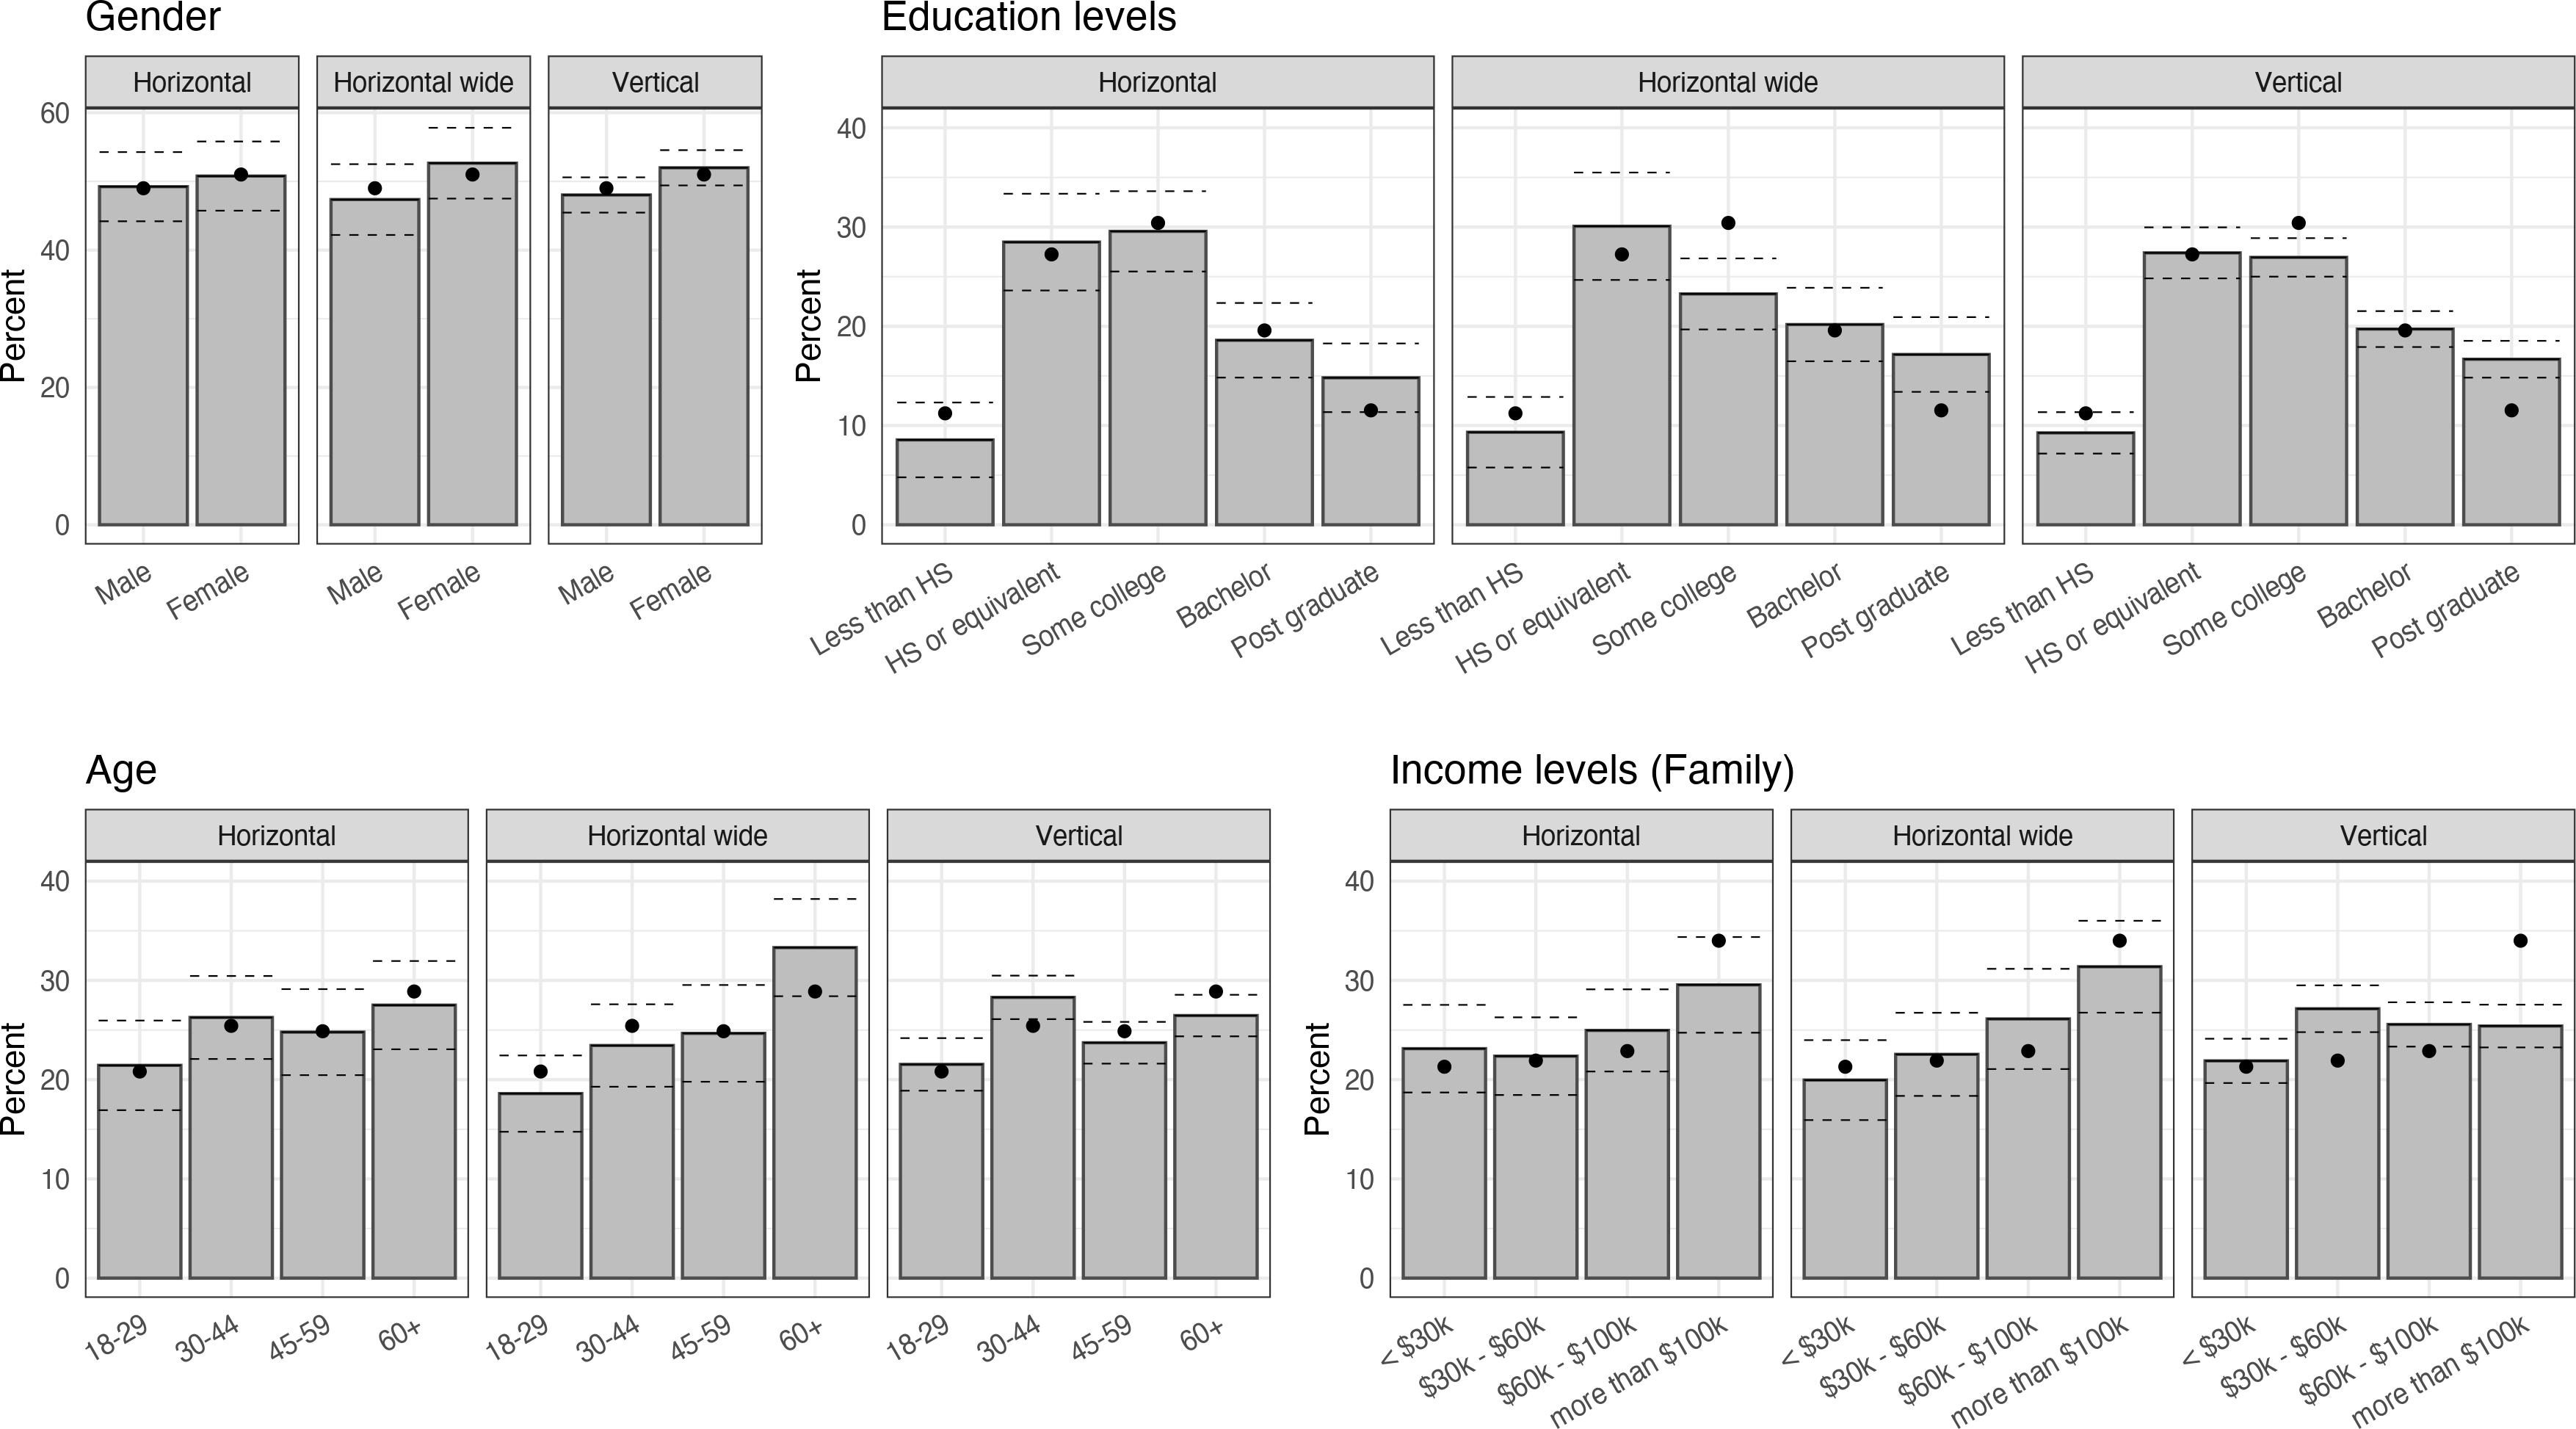
\includegraphics{./figures/fig-rounds-demographics-1.png}

}

\caption{\label{fig-rounds-demographics}Demographics of respondents in
each of the tasks. The dots show percentages of the national
demographics as estimated by the American Community Survery (ACS) 2021.}

\end{figure*}

\hypertarget{accuracy-of-responses}{%
\subsubsection{Accuracy of responses}\label{accuracy-of-responses}}

We first investigate respondent accuracy in selecting the correct
response. As participants were able to select the option `They are the
same', there are several ways to model accuracy and response. The
argument could be made that for the purposes of practical
interpretation, `they are the same' is a correct choice, as the options
are visually very similar and not substantially different values within
the context of the data shown in the chart. However, we are interested
in understanding whether viewers \emph{can} perceive the difference and
correctly identify which piece is larger and thus consider multiple ways
of modeling response to investigate participant response patterns. We
begin by defining a measure of binary `correctness', for which all
answers that are not the correct option (B {[}D{]} is bigger) are
`incorrect', including the selection of `they are the same'.

\autoref{fig-alignment}(a) displays all responses along the binary
correctness measure, separated by whether the stimulus was an aligned
task or unaligned task. We can see that levels of accuracy for all
responses are significantly higher for the `easier' (aligned) task, with
about twice as many respondents correctly selecting the larger of the
two marked elements.

Because each participant was shown both the aligned and unaligned
versions of the chart, we can use a paired \(t\)-test to compare mean
accuracy between the two charts. The resulting \(t\)-statistic is highly
significant (\(t\) statistic: 21.2, df: 2265, \(p\)-value:
\(\ll 0.0001\)).

\begin{figure*}[hbt]

{\centering 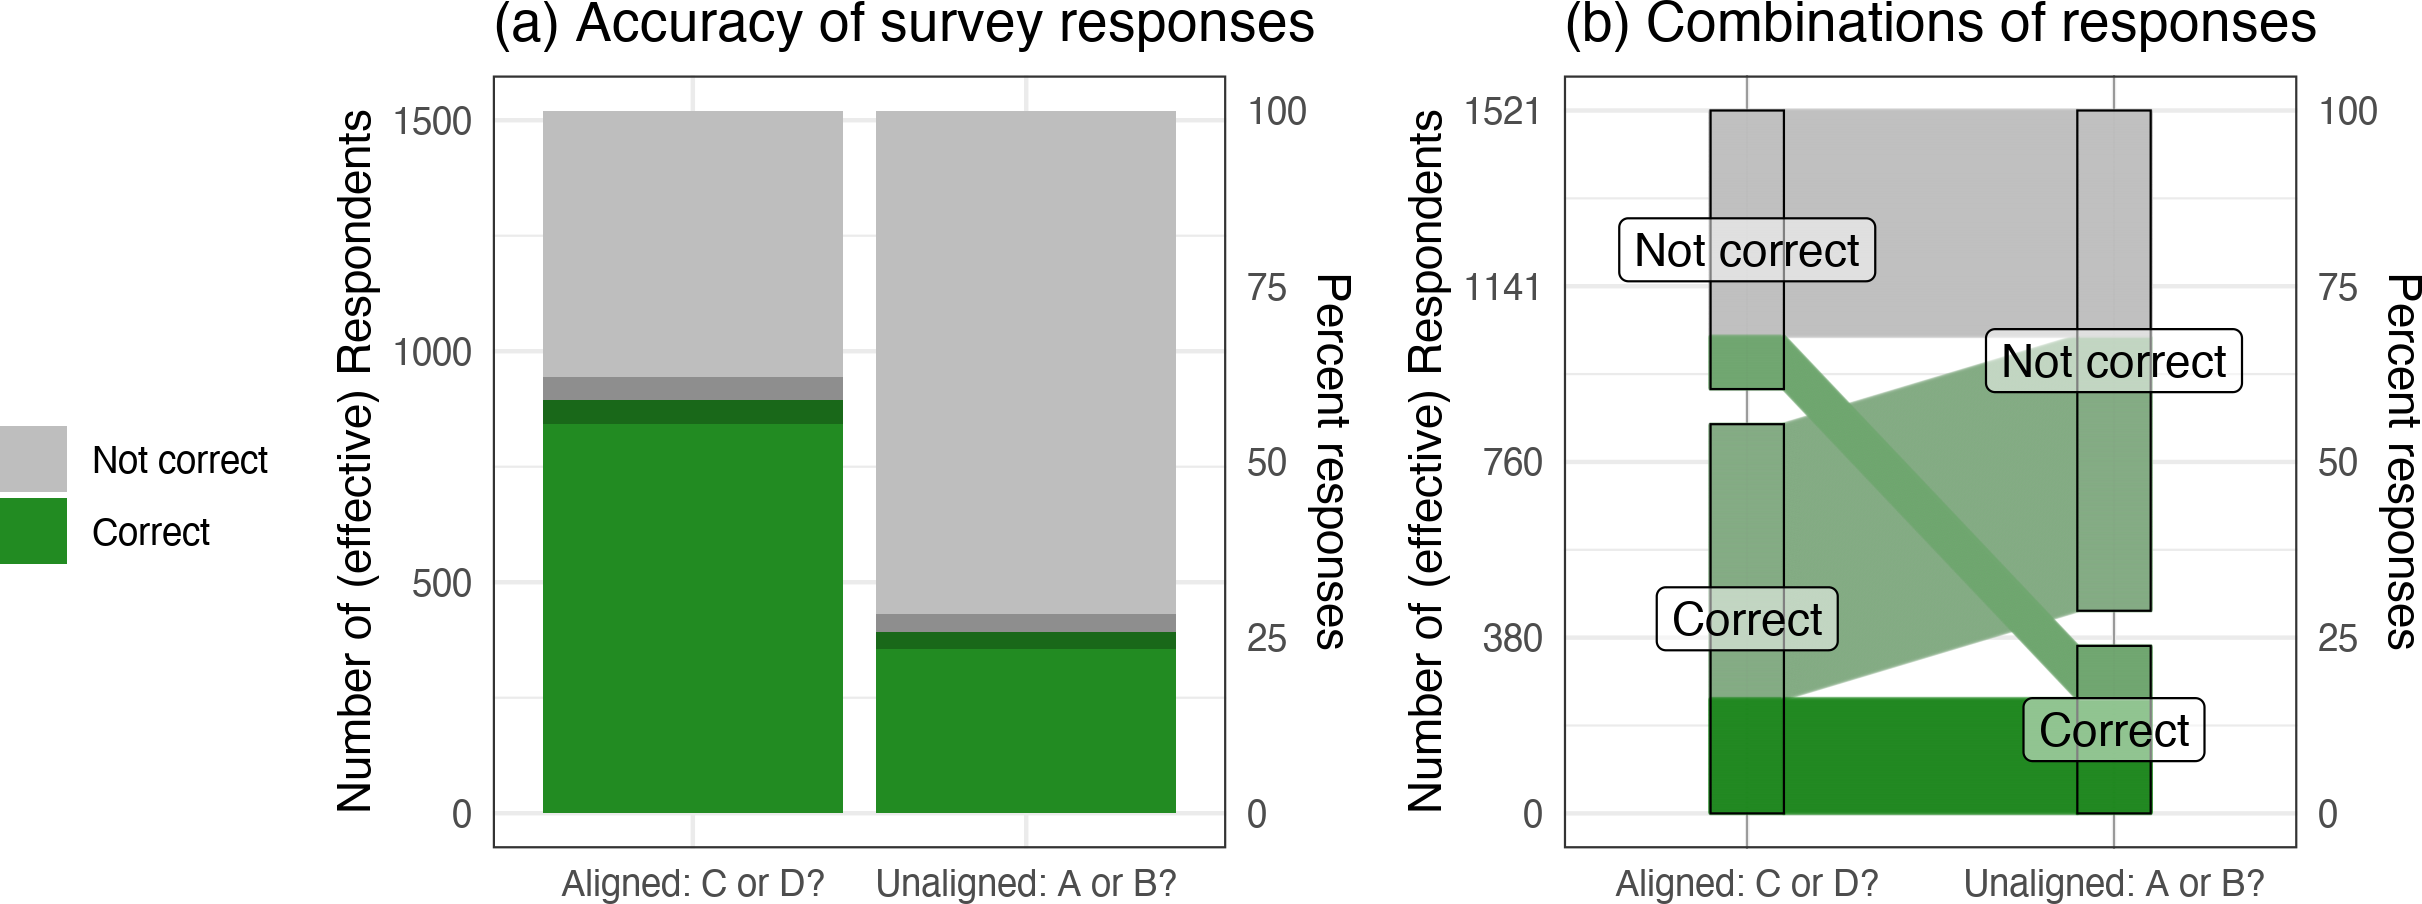
\includegraphics[width=0.9\textwidth,height=\textheight]{./figures/fig-alignment-1.png}

}

\caption{\label{fig-alignment}On the left (a), a stacked barchart shows
the number of respondents with correct (green) and incorrect (grey)
responses to the two comparison questions. When tiles are aligned along
the same axis, more than twice the number of responses are correct. The
shaded area along the top of the green bars corresponds to 95\%
confidence intervals around (marginal) correct responses. On the right
(b), a parallel coordinate plot shows all combinations of responses.
There's a huge asymmetry in the number of responses where participants
answered only one of the questions correctly.}

\end{figure*}

Next, we consider an ordinal model to investigate response behavior
across all three options -- `A {[}C{]} is bigger', `B {[}D{]} is
bigger', and `They are the same', and consider these response patterns
across each of the stimuli.

\begin{figure*}[hbt]

{\centering 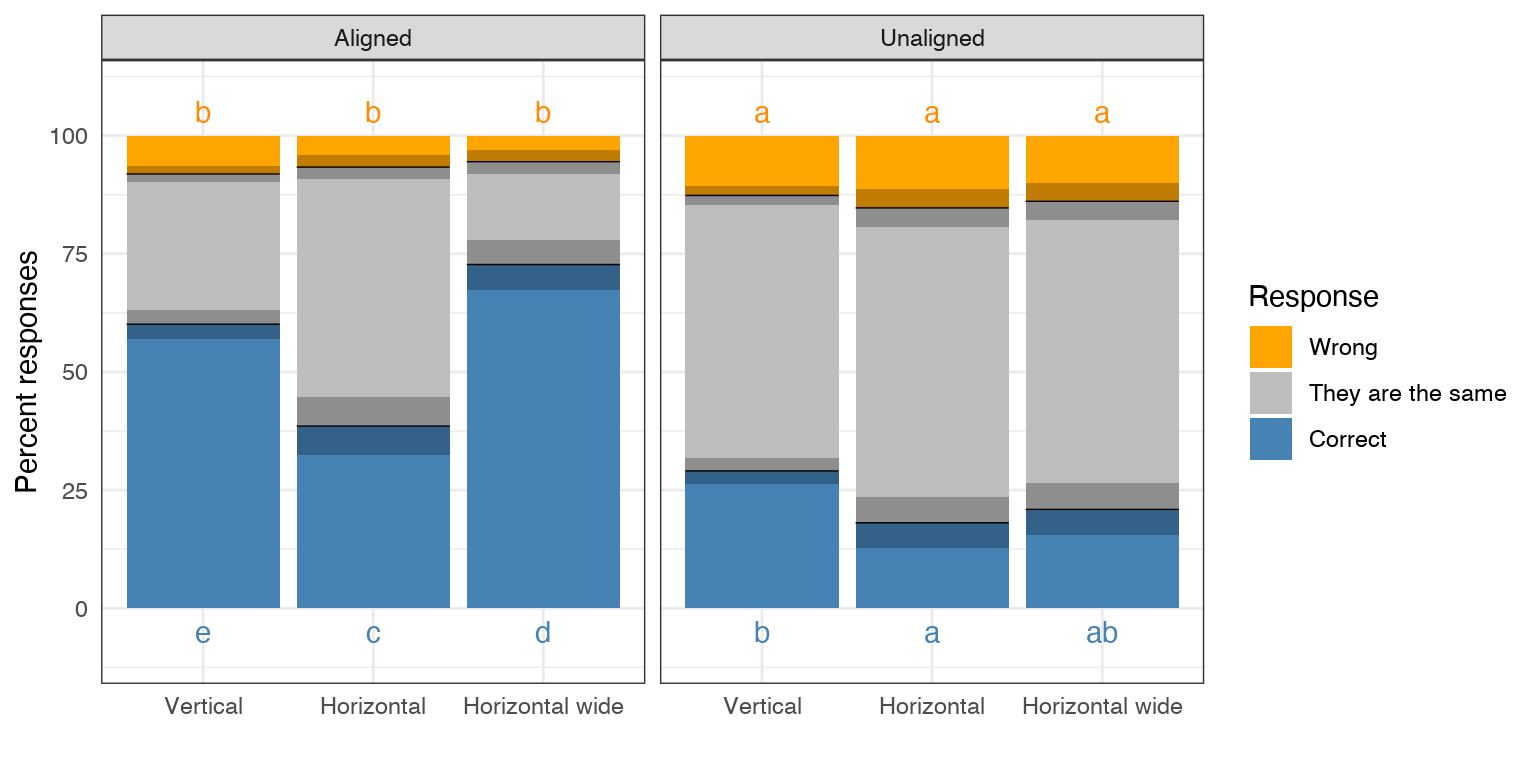
\includegraphics[width=0.9\textwidth,height=\textheight]{./figures/fig-response-123-1.png}

}

\caption{\label{fig-response-123}Responses by task across the designs.
The overlaid rectangles represent 95\% confidence intervals. The letters
in blue and orange encode significances between pairwise proportions:
two bars have a significantly different proportion (at a 5\%
significance level) if they do not share a letter. There is no
significant difference between the designs for wrong responses.}

\end{figure*}

Figure~\ref{fig-response-123} shows the results of a cell-means model
with ordinal response \(Y_k\), where \(Y_k\) is the \(k\)th
participant's response, \(Y_k \in \{1, 2, 3\}\), where `correct' is
encoded as 1, `they are the same' is encoded as 2, and `wrong' is
encoded as 3:

\begin{equation}
\text{logit }P(Y_k \le \ell) = \mu_{ij\ell(k)},
\end{equation}

where \(\ell \in \{1, 2\}\); \(i \in \{1, 2\}\) is the comparison type
(1 = Aligned, 2 = Unaligned), and \(j \in \{1, 2, 3\}\) is the chart
design, with 1 = Vertical, 2 = Horizontal, and 3 = Horizontal wide. The
estimated values and 95\% confidence intervals are shown in
Table~\ref{tbl-rounds-123}. The lowercase letters indicate significances
between pairs of estimates: two estimates within the same column are
significantly different at 5\% level if they do not have any letter in
common (Piepho 2004).

\hypertarget{tbl-rounds-123}{}
\begin{longtable}{lrrlrrl}
\caption{\label{tbl-rounds-123}Estimated odds from the cell-means model for response patterns. Letters
behind numbers indicate pairwise significances. Within the same column,
values are significantly different (at 5\%) if they do not share the
same letter. }\tabularnewline

\caption*{
{\large Odds of selecting responses by task and chart type}
} \\ 
\toprule
 & \multicolumn{3}{c}{correct | same or wrong} & \multicolumn{3}{c}{correct or same | wrong} \\ 
\cmidrule(lr){2-4} \cmidrule(lr){5-7}
 & Est. &           [95\% CI] &   & Est. &           [95\% CI] &   \\ 
\midrule
\multicolumn{7}{l}{Unaligned} \\ 
\midrule
Horizontal & $0.22$ &  [$0.15$, $0.32$] & a & $5.54$ &  [$4.04$, $7.59$] & a \\ 
Horizontal wide & $0.26$ &  [$0.19$, $0.37$] & ab & $6.20$ &  [$4.46$, $8.61$] & a \\ 
Vertical & $0.41$ &  [$0.36$, $0.47$] & b & $6.90$ &  [$5.75$, $8.28$] & a \\ 
\midrule
\multicolumn{7}{l}{Aligned} \\ 
\midrule
Horizontal & $0.63$ &  [$0.49$, $0.81$] & c & $14.02$ &  [$9.23$, $21.30$] & b \\ 
Horizontal wide & $2.67$ &  [$2.04$, $3.48$] & d & $17.12$ &  [$10.49$, $27.95$] & b \\ 
Vertical & $1.51$ &  [$1.33$, $1.71$] & e & $11.33$ &  [$8.99$, $14.28$] & b \\ 
\bottomrule
\end{longtable}

One pattern in accuracy holds across each of the three structural
variations: \textbf{the aligned task has a higher level of accuracy than
its unaligned counterpart}. Interestingly, while we expect an
improvement in accuracy when shifting from the horizontal to the
horizontal wide design given the larger difference in pixel length
between the two pieces, the resulting effects on the accuracy of the
responses are not completely straightforward: the shift from a vertical
to the (tall) horizontal design is detrimental to an accurate perception
for both aligned and unaligned comparisons. The re-scaled design of the
wide horizontal bars reclaims some of the loss for unaligned bars and
outperforms the vertical design by a similar margin in aligned bars, but
does not out-perform the vertical design when comparing unaligned tiles.

Rates of selecting the incorrect response are low across all three
structural variations and the aligned and unaligned tasks; while viewers
select the incorrect response at significantly higher rates for all
three unaligned tasks relative to the aligned tasks, those rates do not
differ significantly across the three structural variations. Most of the
observed differences in response patterns across structural variations
are attributed to respondents' selection between the correct option or
the `they are the same' option.

To better comprehend these observed patterns, we investigate viewer
interaction with the tasks more broadly as well as differences in
response selection across demographic groups.

\hypertarget{respondent-behavior}{%
\subsubsection{Respondent behavior}\label{respondent-behavior}}

One contributing factor to the observed patterns in response accuracy
might be the way that participants interact with the different designs.
Across all tasks, about half of all participants make use of the option
to zoom into charts. We observe that while zooming does help with the
overall accuracy (which is in agreement with the findings by Lu et al.
(2022) about the physical size of stimuli), the increase is not
significant. However, different designs lead to different rates of
zooming: we observe in \autoref{fig-zoom-123} that when dealing with the
vertical design, the rate of zooming is significantly higher than for
the two horizontal designs.

\begin{figure*}[hbt]

{\centering 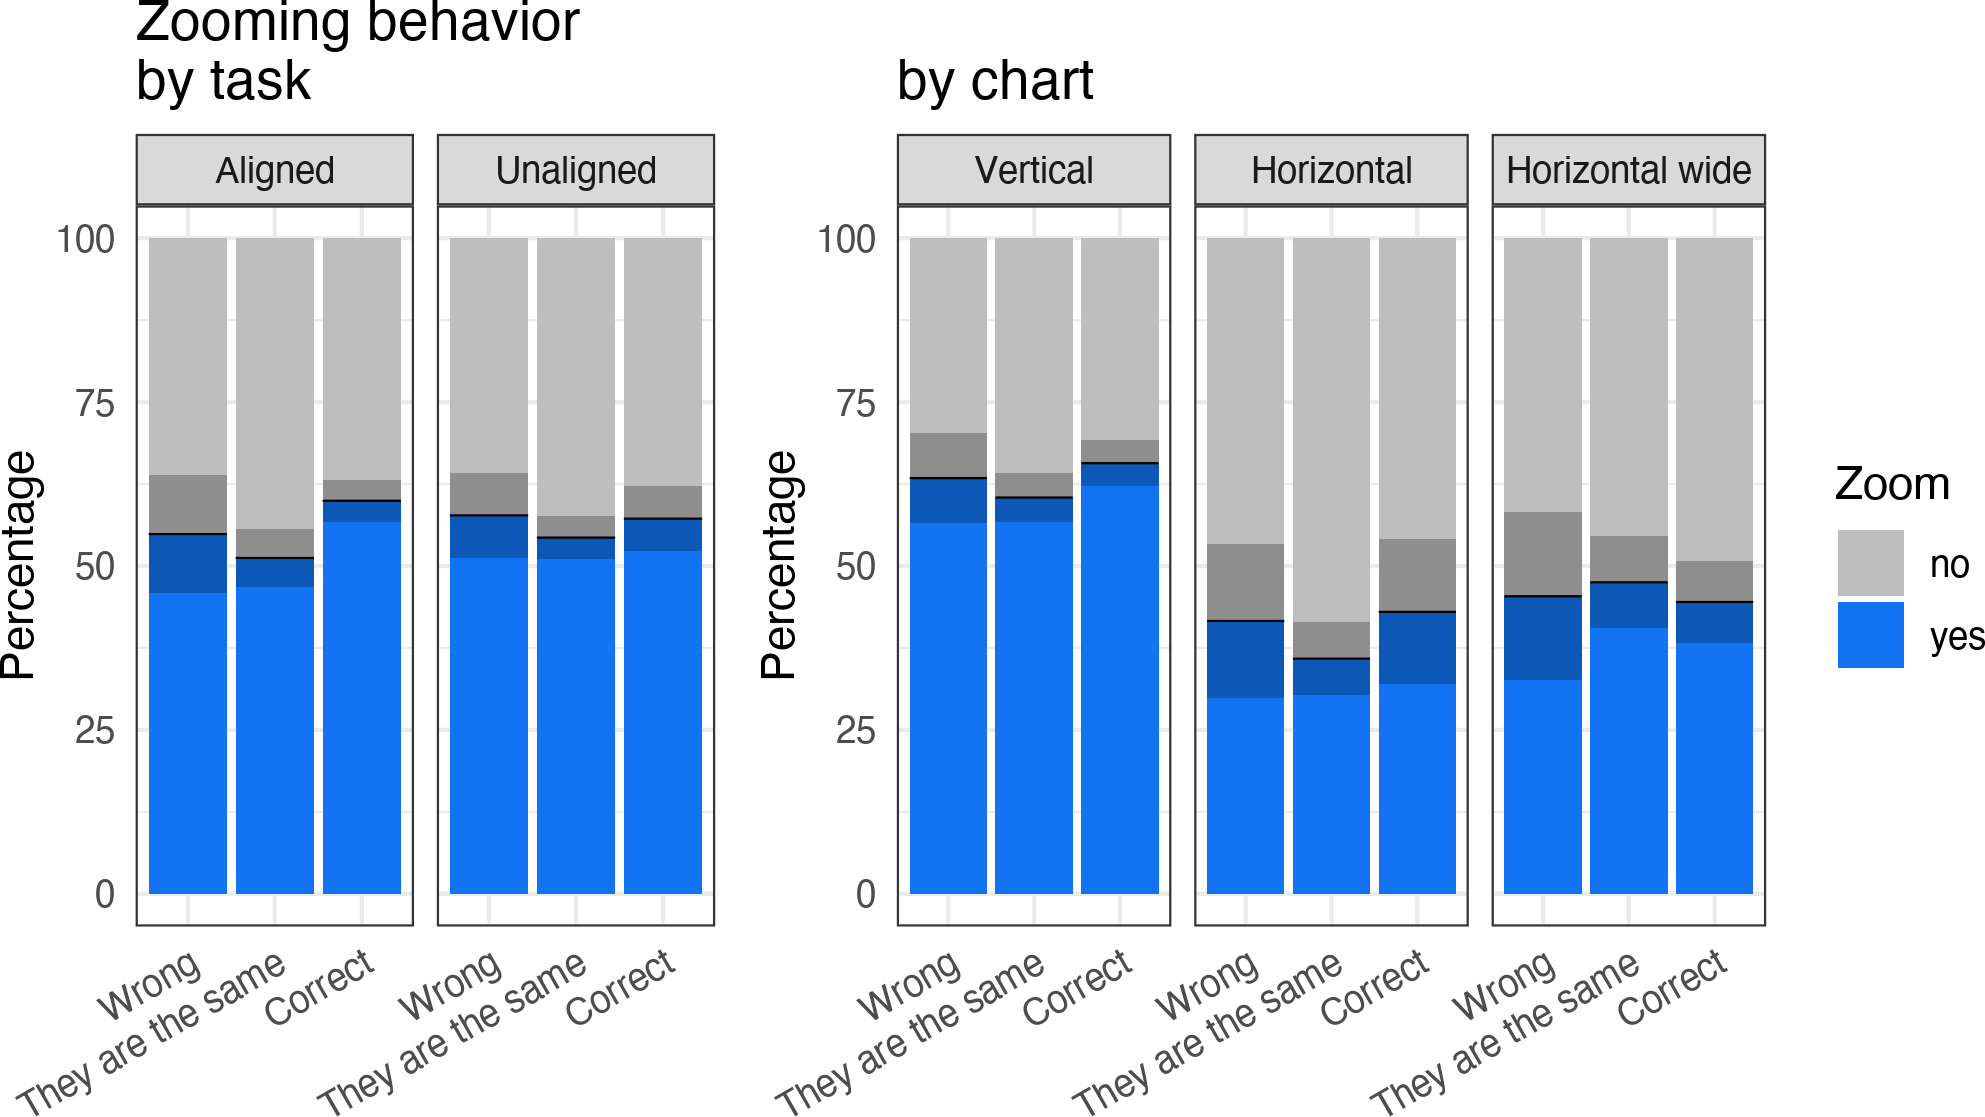
\includegraphics[width=0.8\textwidth,height=\textheight]{./figures/fig-zoom-123-1.png}

}

\caption{\label{fig-zoom-123}Rates of zooming by task, chart design, and
correctness. The overlaid rectangles represent 95\% confidence
intervals. There are significantly higher rates of zooming by
respondents for the vertical task compared to both horizontal tasks;
rates of zooming do not differ by correctness of response or alignment
in the stimulus.}

\end{figure*}

\hypertarget{tbl-zoom-123}{}
\begin{longtable}{lrrrr}
\caption{\label{tbl-zoom-123}Coefficients for logistic regression of zooming by task }\tabularnewline

\caption*{
{\large Estimates for logistic regression on zooming behavior}
} \\ 
\toprule
term & estimate & SE & t-statistic & p-value \\ 
\midrule
\multicolumn{5}{l}{} \\ 
\midrule
\$\$\textbackslash{}hat\{\textbackslash{}mu\}\$\$ & $-0.35$ & $0.15$ & $-2.4$ & 0.0155 \\ 
\midrule
\multicolumn{5}{l}{Response} \\ 
\midrule
\$\$\textbackslash{}text\{They are the same \} \textbackslash{}widehat\{\textbackslash{}rho\}\_\{2\}\$\$ & $-0.17$ & $0.09$ & $-1.9$ & 0.0578 \\ 
Wrong \$\$\textbackslash{}widehat\{\textbackslash{}rho\}\_\{3\}\$\$ & $-0.06$ & $0.13$ & $-0.5$ & 0.6466 \\ 
\midrule
\multicolumn{5}{l}{Task} \\ 
\midrule
Aligned \$\$\textbackslash{}widehat\{\textbackslash{}tau\}\_\{2\}\$\$ & $0.00$ & $0.06$ & $-0.1$ & 0.9435 \\ 
\midrule
\multicolumn{5}{l}{Chart design} \\ 
\midrule
Horizontal wide \$\$\textbackslash{}widehat\{\textbackslash{}delta\}\_\{2\}\$\$ & $0.27$ & $0.15$ & $1.8$ & 0.0752 \\ 
Vertical \$\$\textbackslash{}widehat\{\textbackslash{}delta\}\_\{3\}\$\$ & $0.98$ & $0.13$ & $7.7$ & < 0.0001 \\ 
\bottomrule
\end{longtable}

To formalize this pattern in a model, let \(Y_{jk}\) describe the
zooming behavior of panelist \(k\) on task \(j\). We model zooming
behavior (no = 0, yes = 1) as a logistic regression by correctness of
response (\(\rho\)), task (\(\tau\)), and design (\(\delta\)) of the
chart:

\begin{equation}
\text{logit } P(Y_k \le 1) = \mu + \rho_{i(k)} + \tau_{j(k)} + \delta_{\ell(k)},
\end{equation}

The resulting model estimates and confidence intervals are displayed in
\autoref{tbl-zoom-123}. We observe that zooming behavior \emph{only}
differs significantly by structural design; rates do not differ
significantly between the aligned and unaligned tasks, nor do they
differ significantly by the chosen response. This higher rate of zooming
does not necessarily lead to higher accuracy; although rates of accuracy
are significantly higher for the vertical orientation relative to the
horizontal orientation, they are not significantly higher -- and in
fact, are significantly lower on the aligned task -- than the accuracy
for the horizontal wide orientation.

Using linear scores for the response of certainty, with `not certain at
all' assigned a score of 1 and `extremely certain' assigned a score of
5, we can estimate the effects of task, chart design, and correctness on
certainty by using a cell-means model of the form: \begin{equation}
Y_{k} = \mu_{ij\ell(k)} + \epsilon_{k},
\end{equation} where \(k = 1, ..., N\), \(\mu_{ij\ell(k)}\) is average
certainty (measured on a scale from 1 to 5) of the four combinations of
task and correctness by each of the three designs, where \(i = 1, 2\)
encodes unaligned/aligned, and \(j=1,2\) encodes wrong, correct, and
\(\ell = 1, 2, 3\) encodes horizontal, wide horizontal, and vertical
stacked bar charts, respectively. We also assume that errors are
normally distributed,
i.e.~\(\epsilon_k \stackrel{i.i.d}{\sim} N(0, \sigma^2)\) for all
\(k = 1, ..., N\). The results are shown in Figure~\ref{fig-certainty}.
We find that the highest scores for certainty are associated with the
aligned task, but certainty scores are not significantly different
between correct and wrong responses. Scores are (mostly) significantly
lower for the unaligned task. Interestingly, the lowest certainty scores
are associated with correct responses to the unaligned task; although
respondents successfully complete the task, they are less certain in
their selection.

\begin{figure*}[hbt]

{\centering 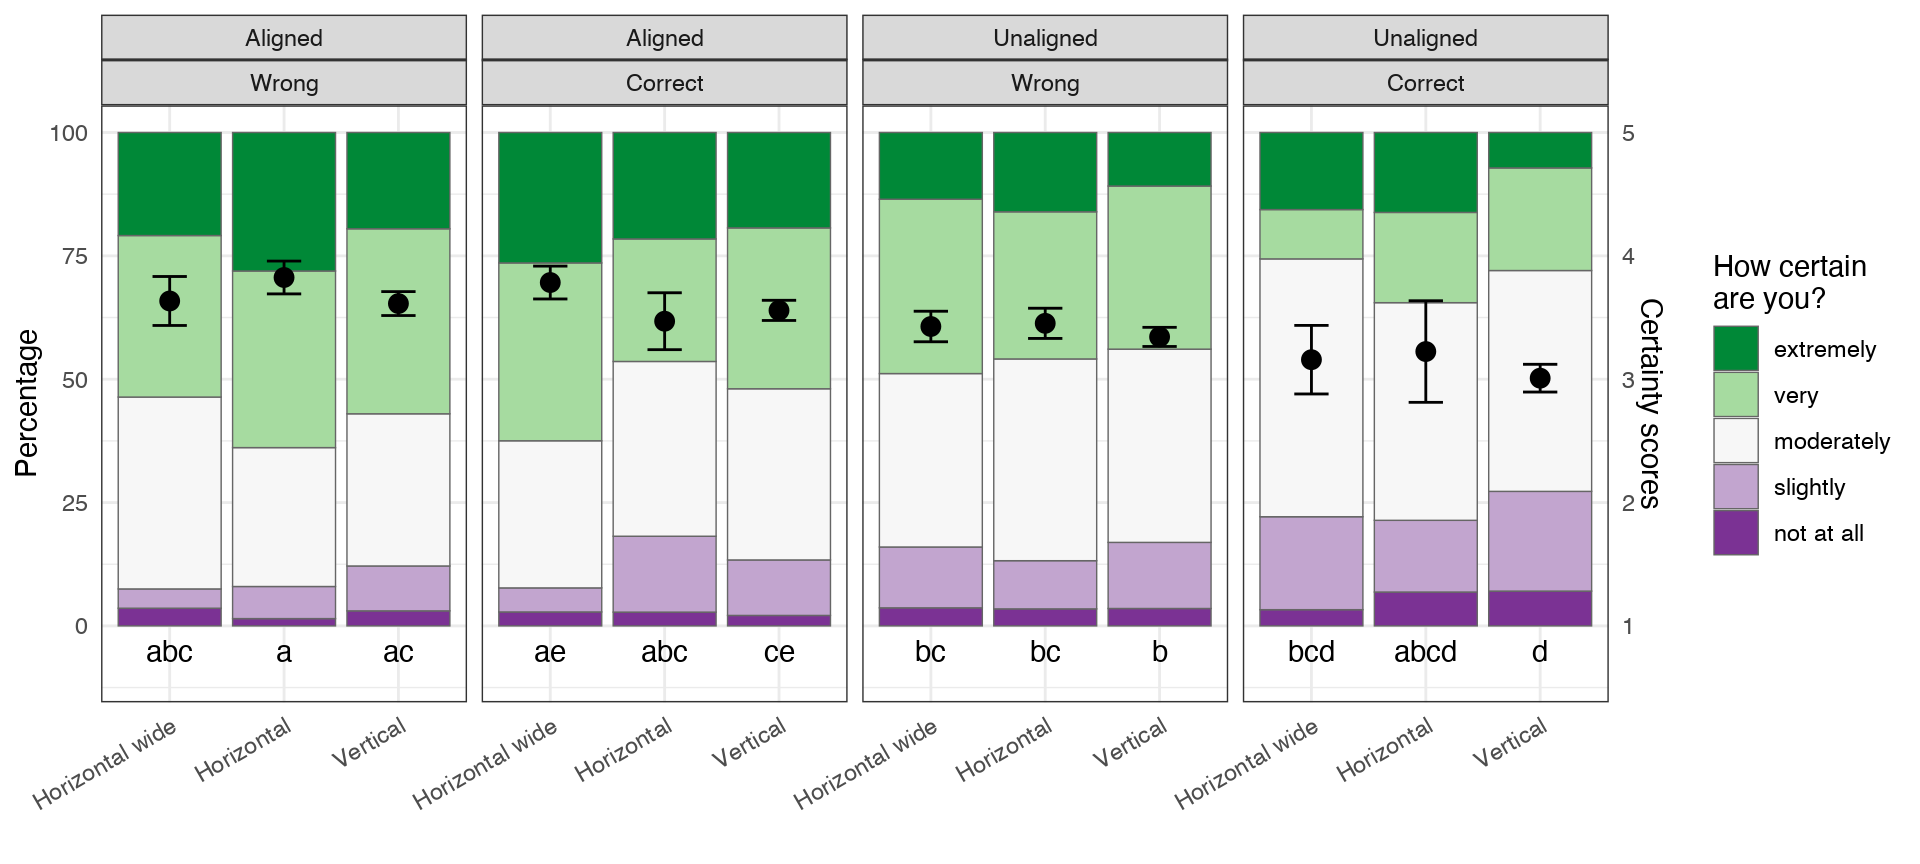
\includegraphics[width=1\textwidth,height=\textheight]{./figures/fig-certainty-1.png}

}

\caption{\label{fig-certainty}Certainty by task, chart design, and
correctness. Correct answers in the unaligned task have the lowest
certainty scores associated with them. Incorrect responses on the
unaligned task show a significant boost in certainty in the vertical
stacked bar. For horizontal stacked bars the difference between aligned
and unaligned charts matters significantly. Error bars around the points
show estimated scores (on a scale of 1 to 5) with corresponding 95\% CI.
The letters underneath the bars indicate significance at 5\%. The scores
for two bars are significantly different if they do not share a letter.}

\end{figure*}

\hypertarget{differences-across-demographic-groups}{%
\subsubsection{Differences across demographic
groups}\label{differences-across-demographic-groups}}

Finally, we turn to investigating responses across demographic groups, a
core benefit provided by the large and representative nature of our
survey samples. \autoref{fig-demographics} displays response patterns
across our three structural variations by gender, age (4 groups),
educational attainment (5 groups), and income level (4 groups). Our
pattern of higher accuracy in selecting the correct response on the
aligned task relative to the unaligned task holds across all demographic
groups and structural variations. However, we do observe different
response patterns, particularly on the unaligned task, across
demographic groups.

Let \(Y_k\) be the response of participant \(k\), on a scale from 1 =
`wrong', 2 = `they are the same' to 3 = `correct'. We use a generalized
cumulative logistic regression, where \(\mu_i\) are intercepts
\(1 \le i < 3\), \(X_k\) are demographics of the \(k\)th participant (in
form of the model matrix), and \(\beta_{i}\) are the coefficients.

\begin{equation}
\text{ logit } P(Y_k \le i \mid X_k) = \mu_i + X_{k}'\beta_{i}
\end{equation}

The resulting model estimates and confidence intervals are shown in
\autoref{tbl-demographics}. When considering the easier (aligned) task,
response patterns do not differ significantly by age, gender, or
education level. We do observe, however, a significantly higher log odds
of selecting the `correct' or `they are the same' response (or
significantly lower log odds of selecting `incorrect') among those with
an income between \$60,000 and \$100,000. When we consider the more
difficult (unaligned) task, we see significant separation in response
patterns across gender, educational attainment, and income groups. We do
not see significant differences in responses by age for either task.
Interestingly, we see lower log odds of selecting the `correct' response
among those with higher educational attainment (those with a bachelor's
degree or post graduate study) \emph{and} lower log odds of selecting
the `incorrect' response; as income and educational attainment increase,
respondents are more likely to select the `they are the same' option
during the difficult task. This speaks to the difficulty of the task,
and respondents' interpretation of the task when it is more difficult to
perceive small differences.

\begin{figure}

\begin{minipage}[t]{\linewidth}

{\centering 

\raisebox{-\height}{

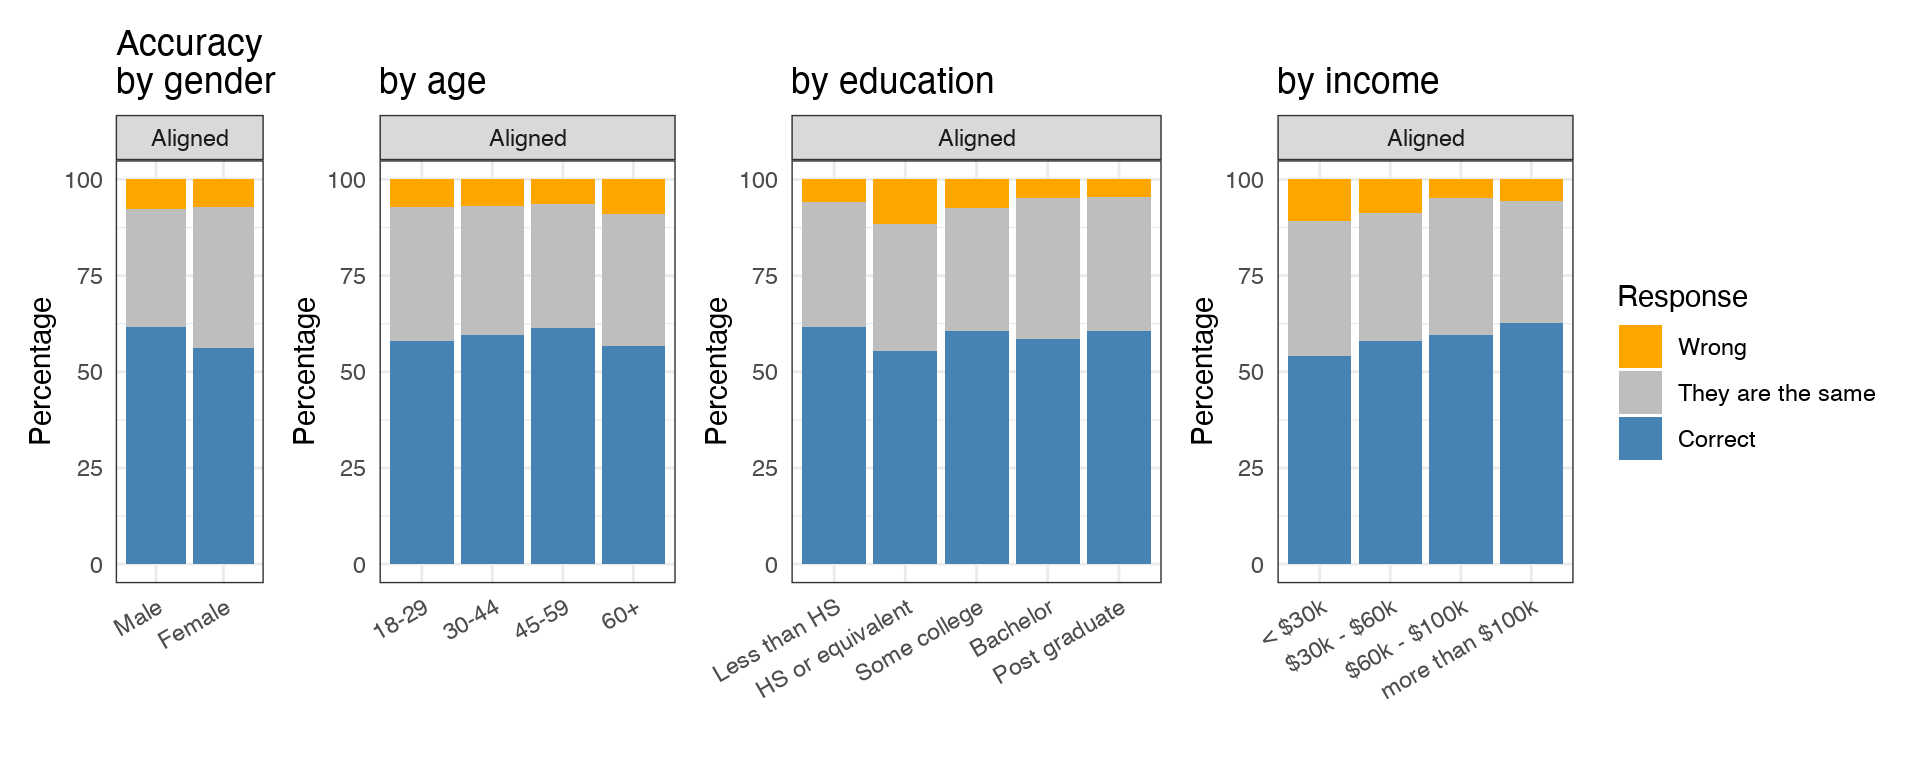
\includegraphics{./figures/fig-demographics-1.png}

}

}

\subcaption{\label{fig-demographics-1}Comparisons of aligned tiles}
\end{minipage}%
\newline
\begin{minipage}[t]{\linewidth}

{\centering 

\raisebox{-\height}{

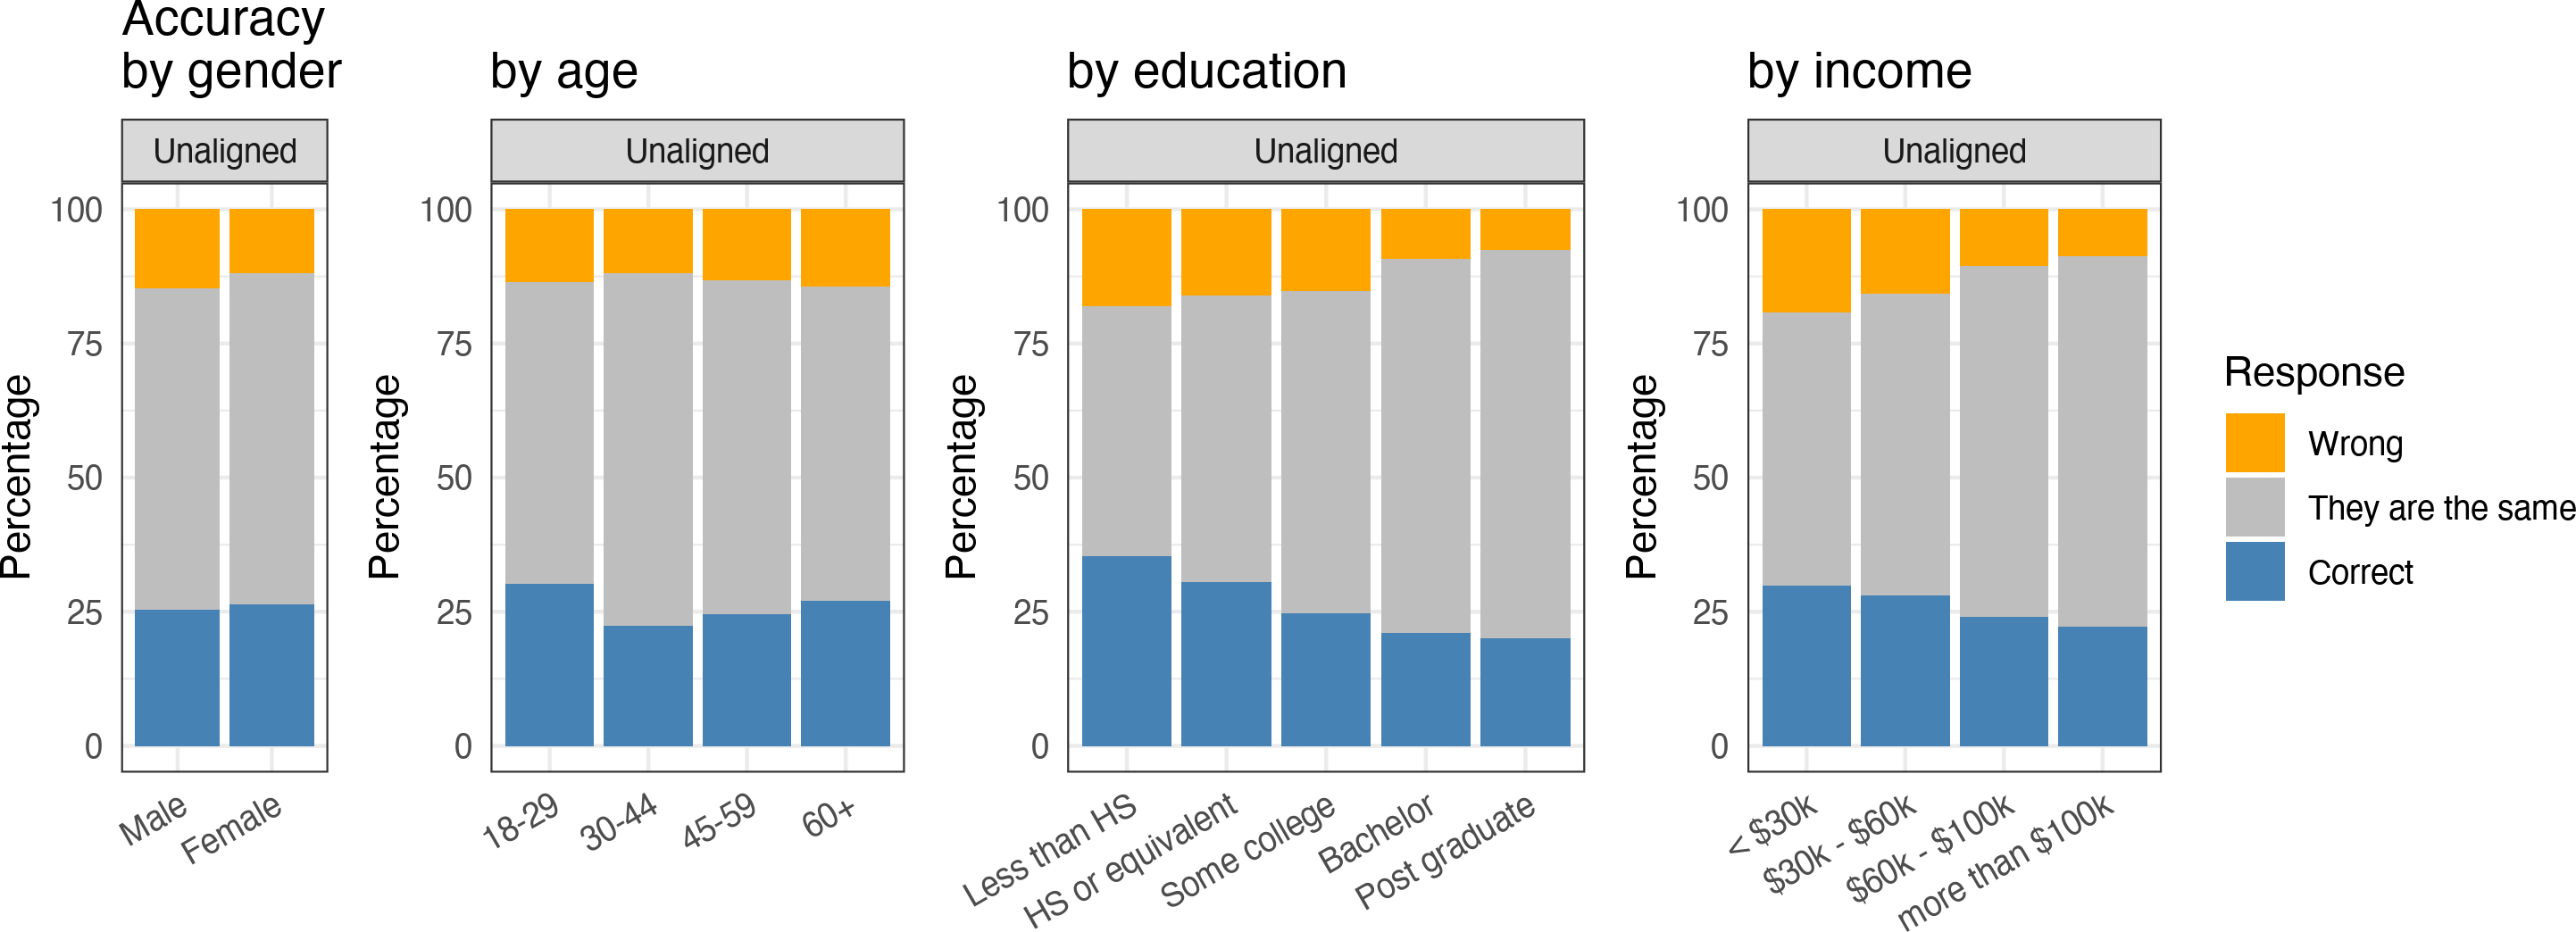
\includegraphics{./figures/fig-demographics-2.png}

}

}

\subcaption{\label{fig-demographics-2}Comparisons of unaligned tiles}
\end{minipage}%

\caption{\label{fig-demographics}Response patterns by alignment and
demographic levels. For aligned tiles, gender, age, and education are
not significant factors. However, income levels do have a (small)
effect. When income levels increase, the percentage of wrong answers
decreases, while the percentage of correct answers increases slightly
(significant at 5\%). For the more difficult task of comparing unaligned
tiles, higher levels of education and higher levels of income are
associated with a significant increase of panelists choosing a response
of `they are the same', resulting in significant decreases of both
correct answers and wrong answers.}

\end{figure}

\blandscape

\hypertarget{tbl-demographics}{}
\setlength{\LTpost}{0mm}
\begin{longtable}{lrrlrrlrrlrrl}
\caption{\label{tbl-demographics}Demographics matter for perception, particularly when the tasks get
harder. }\tabularnewline

\caption*{
{\large Odds of accuracy by task and demographics of respondents}
} \\ 
\toprule
 & \multicolumn{6}{c}{Aligned tiles} & \multicolumn{6}{c}{Unaligned tiles} \\ 
\cmidrule(lr){2-7} \cmidrule(lr){8-13}
 & \multicolumn{3}{c}{correct | same or wrong} & \multicolumn{3}{c}{correct or same | wrong} & \multicolumn{3}{c}{correct | same or wrong } & \multicolumn{3}{c}{correct or same | wrong } \\ 
\cmidrule(lr){2-4} \cmidrule(lr){5-7} \cmidrule(lr){8-10} \cmidrule(lr){11-13}
  & Est. &           [95\% CI] &   & Est. &           [95\% CI] &   & Est. &           [95\% CI] &   & Est. &           [95\% CI] &   \\ 
\midrule
\multicolumn{13}{l}{Intercept} \\ 
\midrule
 & $1.51$ &  [$0.91$, $2.50$] &  & $12.75$ &  [$5.59$, $29.10$] & *** & $0.60$ &  [$0.35$, $1.03$] & . & $3.24$ &  [$1.70$, $6.19$] & *** \\ 
\midrule
\multicolumn{13}{l}{Gender} \\ 
\midrule
Female & $0.82$ &  [$0.67$, $1.01$] & . & $1.19$ &  [$0.81$, $1.74$] &  & $1.03$ &  [$0.82$, $1.30$] &  & $1.42$ &  [$1.07$, $1.90$] & * \\ 
\midrule
\multicolumn{13}{l}{Age} \\ 
\midrule
30-44 & $1.08$ &  [$0.78$, $1.49$] &  & $0.87$ &  [$0.43$, $1.75$] &  & $0.79$ &  [$0.55$, $1.13$] &  & $0.94$ &  [$0.59$, $1.49$] &  \\ 
45-59 & $1.13$ &  [$0.80$, $1.60$] &  & $0.95$ &  [$0.46$, $1.95$] &  & $0.92$ &  [$0.62$, $1.35$] &  & $0.76$ &  [$0.48$, $1.22$] &  \\ 
60+ & $0.96$ &  [$0.69$, $1.34$] &  & $0.70$ &  [$0.35$, $1.40$] &  & $1.01$ &  [$0.70$, $1.45$] &  & $0.73$ &  [$0.46$, $1.15$] &  \\ 
\midrule
\multicolumn{13}{l}{Education} \\ 
\midrule
HS or equivalent & $0.77$ &  [$0.46$, $1.30$] &  & $0.50$ &  [$0.20$, $1.21$] &  & $0.81$ &  [$0.47$, $1.40$] &  & $1.22$ &  [$0.66$, $2.27$] &  \\ 
Some college & $0.91$ &  [$0.56$, $1.49$] &  & $0.74$ &  [$0.32$, $1.71$] &  & $0.63$ &  [$0.38$, $1.06$] & . & $1.17$ &  [$0.65$, $2.12$] &  \\ 
Bachelor & $0.79$ &  [$0.48$, $1.32$] &  & $1.12$ &  [$0.42$, $2.97$] &  & $0.53$ &  [$0.31$, $0.93$] & * & $1.82$ &  [$0.91$, $3.64$] & . \\ 
Post graduate & $0.84$ &  [$0.49$, $1.44$] &  & $1.16$ &  [$0.41$, $3.30$] &  & $0.51$ &  [$0.28$, $0.91$] & * & $2.18$ &  [$1.04$, $4.57$] & * \\ 
\midrule
\multicolumn{13}{l}{Income} \\ 
\midrule
\$30k - \$60k & $1.19$ &  [$0.87$, $1.63$] &  & $1.25$ &  [$0.77$, $2.05$] &  & $1.00$ &  [$0.71$, $1.41$] &  & $1.22$ &  [$0.82$, $1.82$] &  \\ 
\$60k - \$100k & $1.23$ &  [$0.90$, $1.68$] &  & $2.14$ &  [$1.18$, $3.86$] & * & $0.87$ &  [$0.60$, $1.27$] &  & $1.88$ &  [$1.24$, $2.87$] & ** \\ 
more than \$100k & $1.36$ &  [$0.99$, $1.88$] & . & $1.57$ &  [$0.86$, $2.86$] &  & $0.86$ &  [$0.59$, $1.25$] &  & $2.18$ &  [$1.34$, $3.56$] & ** \\ 
\bottomrule
\end{longtable}
\begin{minipage}{\linewidth}
Signif. codes:  0 `***' 0.001 `**' 0.01 `*' 0.05 `.' 0.1 ` ' 1\\
\end{minipage}

\elandscape

\hypertarget{conclusions}{%
\section{Conclusions}\label{conclusions}}

Through this work, we have tested the use of probability-based survey
panels to ask perception questions; within a large survey covering a
variety of topics, and with a limited number of questions for our
specific tasks, we are able to measure viewer perception and produce
results consistent with prior studies. Testing data visualization design
structures and viewer behavior on a nationally-representative sample is
of broad interest and applicability to the scientific communication
community, and this study demonstrates a framework under which to
complete further work in this area.

With our survey framework, we have shown that we can rank structural
variations on design and tasks by their relative accuracy; we identified
significantly different rates of respondent accuracy under different
designs presenting the same data. The size of our sample aids in
identifying this signal.

Further, we can also study respondent behavior and how viewers interact
with the chart. Paradata on viewer interaction with the chart (e.g.,
zooming and time spent on each task) can be collected as well as asking
directly asking respondents questions about their certainty. Not only
can we collect this information, but we can also identify significant
differences in this behavior across different designs. Understanding
viewer interaction and engagement is a key component to designing
effective data visualizations. If a particular design leads viewers to
zoom in more to investigate it when determining a response, we might
consider that design to be more frustrating to viewers `in the wild'
when viewing it outside of the context of our tests.

Perhaps most salient among our results are the patterns in response
behavior across demographic groups. The large size of our sample, paired
with the probability-based survey panel approach, afford us the ability
to dive into response patterns among demographics across tasks and
identify significant differences among them. In particular, the
differences across educational attainment groups and income groups
underscore the importance of utilizing a representative population when
testing perception; prior results in this area may be absorbing bias in
responses due to the larger representation of individuals with higher
education levels among those study respondents.

Our study results provide actionable insights that data visualization
practitioners can utilize in the design of data visualizations.
Comparisons of interest should be lined up and share a common baseline
within a chart; in an interactive setting, it may be beneficial to give
viewers the possibility of re-ordering categories to support effective
comparison across groupings. Allowing users to zoom in on images may not
impact perceptual accuracy, but it leads to higher certainty in viewers'
comparisons. Considering the target audience for visualizations and what
key findings are most important to convey should be an important step in
the process of designing a data visualization.

While our results are limited to mapping in a stacked bar chart with a
specific topic, they demonstrate among them a wealth of insights about
how respondents perceive and interact with data visualizations. More
expansive work on this topic should be completed to understand how the
general public interacts with and understands charts, including
expanding to a wider set of structural variations, more aesthetic design
variations, and considering differences in respondent behavior across
different data topic areas.

\hypertarget{references}{%
\section*{References}\label{references}}
\addcontentsline{toc}{section}{References}

\hypertarget{refs}{}
\begin{CSLReferences}{1}{0}
\leavevmode\vadjust pre{\hypertarget{ref-borgoCrowdsourcingInformationVisualization2017}{}}%
Borgo, Rita, Bongshin Lee, Benjamin Bach, Sara Fabrikant, Radu Jianu,
Andreas Kerren, Stephen Kobourov, et al. 2017. {``Crowdsourcing for
{Information Visualization}: {Promises} and {Pitfalls}.''} In
\emph{Evaluation in the {Crowd}. {Crowdsourcing} and {Human-Centered
Experiments}}, edited by Daniel Archambault, Helen Purchase, and Tobias
Hoßfeld, 96--138. Lecture {Notes} in {Computer Science}. {Springer
International Publishing}.

\leavevmode\vadjust pre{\hypertarget{ref-clevelandGraphicalPerceptionTheory1984}{}}%
Cleveland, William S., and Robert McGill. 1984. {``Graphical Perception:
{Theory}, Experimentation, and Application to the Development of
Graphical Methods.''} \emph{Journal of the American Statistical
Association} 79 (387): 531--54.
\url{https://doi.org/10.1080/01621459.1984.10478080}.

\leavevmode\vadjust pre{\hypertarget{ref-dennis2019technical}{}}%
Dennis, J Michael. 2019, updated 2022. {``Technical Overview of the
{AmeriSpeak} Panel {NORC}'s Probability-Based Household Panel.''}
\emph{NORC at the University of Chicago}, 2019, updated 2022.

\leavevmode\vadjust pre{\hypertarget{ref-heerCrowdsourcingGraphicalPerception2010}{}}%
Heer, J., and M. Bostock. 2010. {``Crowdsourcing Graphical Perception:
{Using} Mechanical {Turk} to Assess Visualization Design.''} In
\emph{Conference on {Human Factors} in {Computing Systems} -
{Proceedings}}, 1:203--12. {ACM}.
\url{https://doi.org/10.1145/1753326.1753357}.

\leavevmode\vadjust pre{\hypertarget{ref-kishSurveySampling1965}{}}%
Kish, Leslie. 1965. \emph{Survey {Sampling}}. {Wiley}.

\leavevmode\vadjust pre{\hypertarget{ref-luModelingJustNoticeable2022}{}}%
Lu, Min, Joel Lanir, Chufeng Wang, Yucong Yao, Wen Zhang, Oliver
Deussen, and Hui Huang. 2022. {``Modeling {Just Noticeable Differences}
in {Charts}.''} \emph{IEEE Transactions on Visualization and Computer
Graphics} 28 (1): 718--26.
\url{https://doi.org/10.1109/TVCG.2021.3114874}.

\leavevmode\vadjust pre{\hypertarget{ref-lumleyAnalysisComplexSurvey2004}{}}%
Lumley, Thomas. 2004. {``Analysis of Complex Survey Samples.''}
\emph{Journal of Statistical Software} 9 (1): 1--19.

\leavevmode\vadjust pre{\hypertarget{ref-lumleyComplexSurveysGuide2010}{}}%
---------. 2010. \emph{Complex Surveys: {A} Guide to Analysis Using {R}:
{A} Guide to Analysis Using {R}}. {John Wiley and Sons}.

\leavevmode\vadjust pre{\hypertarget{ref-survey}{}}%
---------. 2020. {``Survey: Analysis of Complex Survey Samples.''}

\leavevmode\vadjust pre{\hypertarget{ref-mackinlayAutomatingDesignGraphical1986}{}}%
Mackinlay, Jock. 1986. {``Automating the Design of Graphical
Presentations of Relational Information.''} \emph{ACM Transactions on
Graphics} 5 (2): 110--41. \url{https://doi.org/10.1145/22949.22950}.

\leavevmode\vadjust pre{\hypertarget{ref-omuircheartaighCombiningSamplesVs2002}{}}%
O'Muircheartaigh, Colm, and Steven Pedlow. 2002. {``Combining {Samples
Vs}. {Cumulating Cases}: {A Comparison} of {Two Weighting Strategies} in
{Nlsy97}.''} In \emph{{ASA Proceedings} of the {Joint Statistical
Meetings}}, 2557--62.
\url{http://www.asasrms.org/Proceedings/y2002/Files/JSM2002-001082.pdf}.

\leavevmode\vadjust pre{\hypertarget{ref-piephoAlgorithmLetterBasedRepresentation2004}{}}%
Piepho, Hans-Peter. 2004. {``An {Algorithm} for a {Letter-Based
Representation} of {All-Pairwise Comparisons}.''} \emph{Journal of
Computational and Graphical Statistics} 13 (2): 456--66.
\url{https://doi.org/10.1198/1061860043515}.

\leavevmode\vadjust pre{\hypertarget{ref-RLanguage}{}}%
R Core Team. 2022. \emph{R: {A} Language and Environment for Statistical
Computing}. Manual. {Vienna, Austria}: {R Foundation for Statistical
Computing}. \url{https://www.R-project.org/}.

\leavevmode\vadjust pre{\hypertarget{ref-talbotFourExperimentsPerception2014}{}}%
Talbot, Justin, Vidya Setlur, and Anushka Anand. 2014. {``Four
{Experiments} on the {Perception} of {Bar Charts}.''} \emph{IEEE
Transactions on Visualization and Computer Graphics} 20 (12): 2152--60.
\url{https://doi.org/10.1109/TVCG.2014.2346320}.

\leavevmode\vadjust pre{\hypertarget{ref-zacksReadingBarGraphs1998a}{}}%
Zacks, Jeff, Ellen Levy, Barbara Tversky, and Diane J. Schiano. 1998.
{``Reading Bar Graphs: {Effects} of Extraneous Depth Cues and Graphical
Context.''} \emph{Journal of Experimental Psychology: Applied} 4 (2):
119--38. \url{https://doi.org/10.1037/1076-898X.4.2.119}.

\end{CSLReferences}



\end{document}
